% GRASP: Copyright 1997,1998,1999  Bruce Allen
% $Id: man_template.tex,v 1.11 1999/07/11 21:22:16 ballen Exp $
\section{GRASP Routines: Template Bank Generation \& Searching}
\label{s:template}
\setcounter{equation}0
For the most part, one of our main interests is the search
for signals whose wave-forms are characterized
by unknown values of a set of parameters (for binary inspiral, these
would be $m_1$ and $m_2$).
In order to use the matched filtering technique described in the previous section,
it is necessary to set up a ``bank" of templates, designed so that any
expected signal is ``close" (in parameter space) to one of
the elements of the bank.
This section contains a set of routines for setting up such a template bank,
in the case where the signals are parameterized by two parameters.

It also contains a (parallel) routine to search for binary inspiral
in a bank of templates.
\subsection{Structure: {\tt struct Template}}
\setcounter{equation}0
The structure used to describe the ``chirp" signals from coalescing
binary systems is:
{\tt struct Template} \{
\begin{description}
\item{\tt int num:}
   In order to deal with templates ``wholesale" it is useful to number
   them.  The numbering system is up to you; we typically give each
   template a number, starting from 0 and going up to the number of
   templates minus one!
\item{\tt float f\_lo:}
   This is the starting (low) frequency $f_0$ of template, in units of ${\rm
   sec}^{-1}$.
\item{\tt float f\_hi:}
   This is the ending (high) frequency of the template, in units of
   ${\rm sec}^{-1}$
\item{\tt float tau0:}
   The Newtonian time $\tau_0$ to coalescence, in seconds, starting from the
   moment when the frequency of the waveform is f\_lo.
\item{\tt float tau1:}
   First post-Newtonian correction $\tau_1$ to $\tau_0$. 
\item{\tt float tau15:}
   3/2 PN correction 
\item{\tt float tau20:}
   second order  PN correction 
\item{\tt float pha0:}
   Newtonian phase to coalescence, radians 
\item{\tt float pha1:}
   First post-Newtonian correction to pha0 
\item{\tt float pha15:}
   3/2 PN correction 
\item{\tt float pha20:}
   second order  PN correction 
\item{\tt float mtotal:}
   total mass $m_1+m_2$, in solar masses 
\item{\tt float mchirp:}
   chirp mass $\mu \eta^{-2/5}$, in solar masses 
\item{\tt float mred:}
   the reduced mass $\mu=m_1 m_2/(m_1+m_2)$, in solar masses 
\item{\tt float eta:}
   reduced mass/total mass $\eta=m_1 m_2/(m_1+m_2)^2$ , dimensionless
\item{\tt float m1:}
   the smaller of the two masses, in solar masses.
\item{\tt float m2:}
   the larger of the two masses, in solar masses.
\end{description}
\};

One may use the technique of {\it matched filtering} to search for
chirps.  The (noisy) signal is compared with templates, each formed
from a  chirp with a particular values of $m_1$, $m_2$, and a ``start
frequency" $f_0$  of the waveform at the time that it enters the
bandpass of the gravitational wave detector. Several theoretical
studies \cite{Bala,Owen} have shown how the template filtering
technique performs when the detector is not ideal, but is contaminated by
instrument noise.

In the presence of detector noise, one can never be entirely certain
that a given chirp (determined by $m_1,m_2$) will be detected by a
particular template, even one with the exact same mass parameters.
However one can make statistical statements about a template, such as
``if the masses $m_1$ and $m_2$ of the chirp lie in region $R$ of
parameter space, then with 97\% probability, they will be detected if
their amplitude exceeds value $h$".  Thus, associated with each chirp,
and a specified level of uncertainty, is a region of parameter space.

It turns out that if we use the correct choice of coordinates on the
parameter space $(m_1,m_2)$ then these regions $R$ are quite simple.
If we demand that the uncertainty associated with each template be
fairly small, then these regions are ellipses.  Moreover, to a good
approximation, the shape of the ellipses is determined only by the
noise power spectrum of the detector, and does not change significantly
as we move about in the parameter space.  These ``nice" coordinates
$(\tau_0,\tau_1)$ have units of time, and are defined by
\begin{eqnarray}
\label{e:tau0}
\tau_0 &=& {5 \over 256} \left({ G M \over c^3}\right)^{-5/3} \eta^{-1}
(\pi f_0)^{-8/3} \\
\nonumber
&=& {5 \over 256}  \left({ M \over M_\odot}\right)^{-5/3}\eta^{-1} (\pi
f_0)^{-8/3} T_\odot^{-5/3}
\end{eqnarray}
and 
\begin{eqnarray}
\label{e:tau1}
\tau_1 &=& {5 \over 192} \left({c^3 \over G \eta M }\right) \left({743
\over 336} + {11 \over 4} \eta \right) (\pi f_0)^{-2}\\
\nonumber
&=& {5 \over 192} \left( {M_\odot \over  M }\right) \left({743 \over
336} \eta^{-1} + {11 \over 4} \right) (\pi f_0)^{-2} T_\odot^{-1}.
\end{eqnarray}
The symbol
\begin{equation}
M \equiv m_1+m_2
\end{equation}
denotes the total mass of the binary system, and
\begin{equation}
\eta \equiv {m_1 m_2 \over (m_1 + m_2)^2}
\end{equation}
is the ratio of the reduced
mass to $M$.  Notice that $\eta$ is always (by definition) less than or
equal to $1/4$.

We are generally interested in a region of parameter space
corresponding to binary systems, each of whose masses lie in some given
range, say from $1/2$ to $3$ solar masses.  The region of parameter
space is determined by a minimum and maximum mass; we show an example
of this in Figure \ref{f:massrange}.
\begin{figure}[hb]
\begin{center}
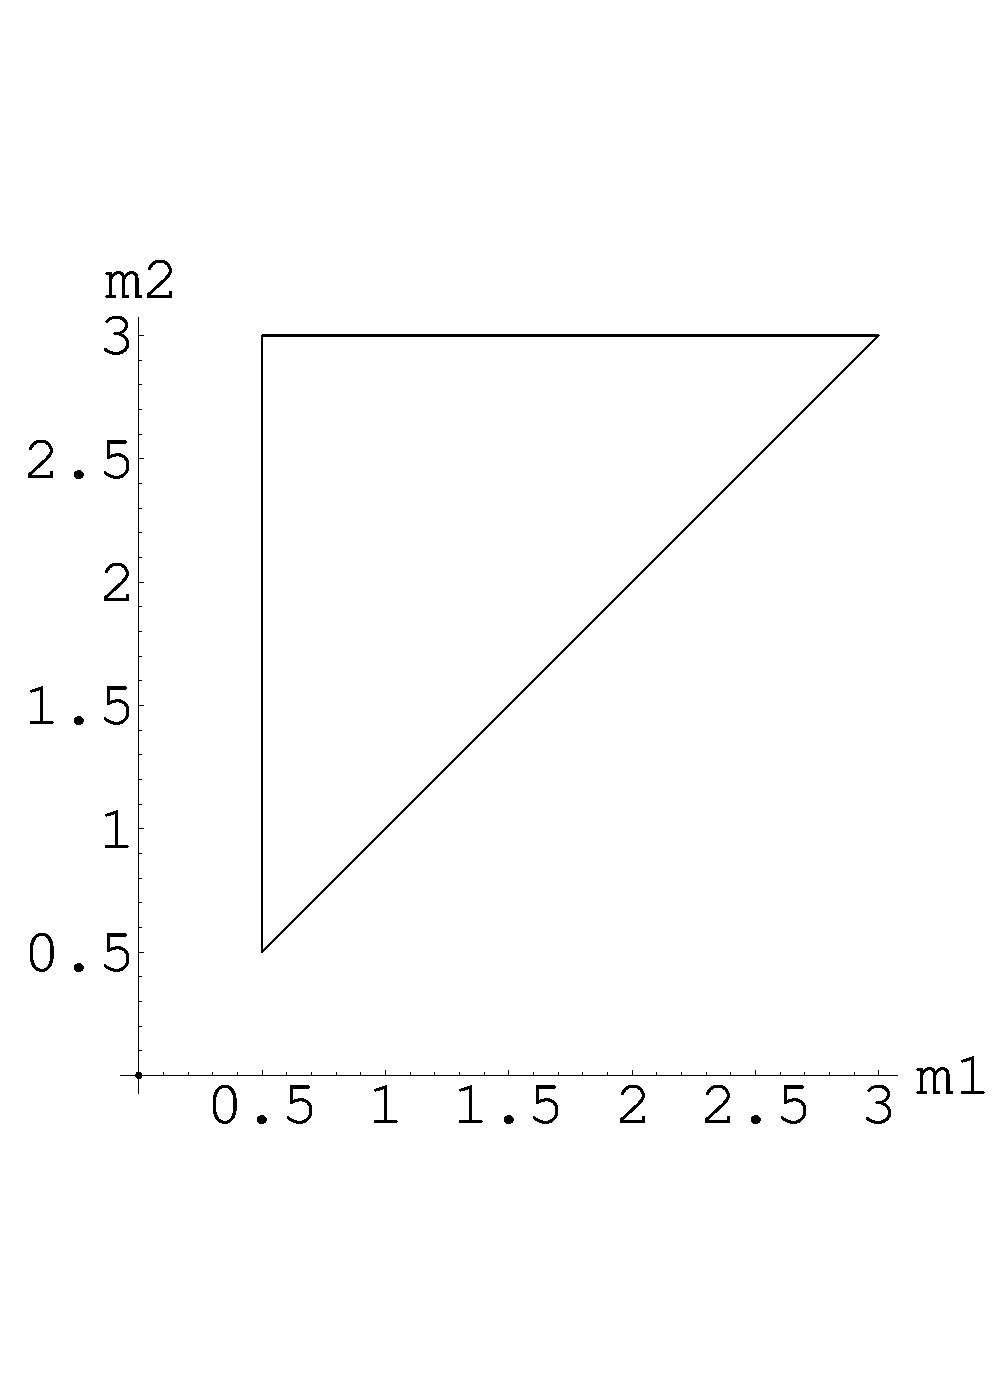
\epsfig{file=Figures/figure1.ps,height=6cm,bbllx=72pt,bblly=160pt,
bburx=540pt,bbury=650pt}
\caption{\label{f:massrange} The set of binary stars with masses lying
between set minimum and maximum values defines the interior of a
triangle in parameter space}
\end{center}
\end{figure}
Since we may take $m_2 \le m_1$ without loss of generality, the region
of interest is triangular rather than rectangular.  The three
lines on this diagram are:
\begin{description}
\item{(1)} The equal mass line.  Along this line $\eta=1/4$.
\item{(2)} The minimum mass line.  Along this line, one of the masses has its smallest value.
\item{(3)} The maximum mass line.  Along this line, one of the masses has its largest value.
\end{description}
This triangular region is mapped into the $(\tau_0,\tau_1)$ plane as
shown in Figure \ref{f:taurange}
In this diagram, the lower curve $\tau_1 \propto \tau_0^{3/5}$ is the
equal mass line (1).  The upper curve, to the right of the ``kink" is
the minimum mass line (2).  The upper curve, to the left of the
``kink" is the maximum mass line (3).
\begin{figure}[hb]
\begin{center}
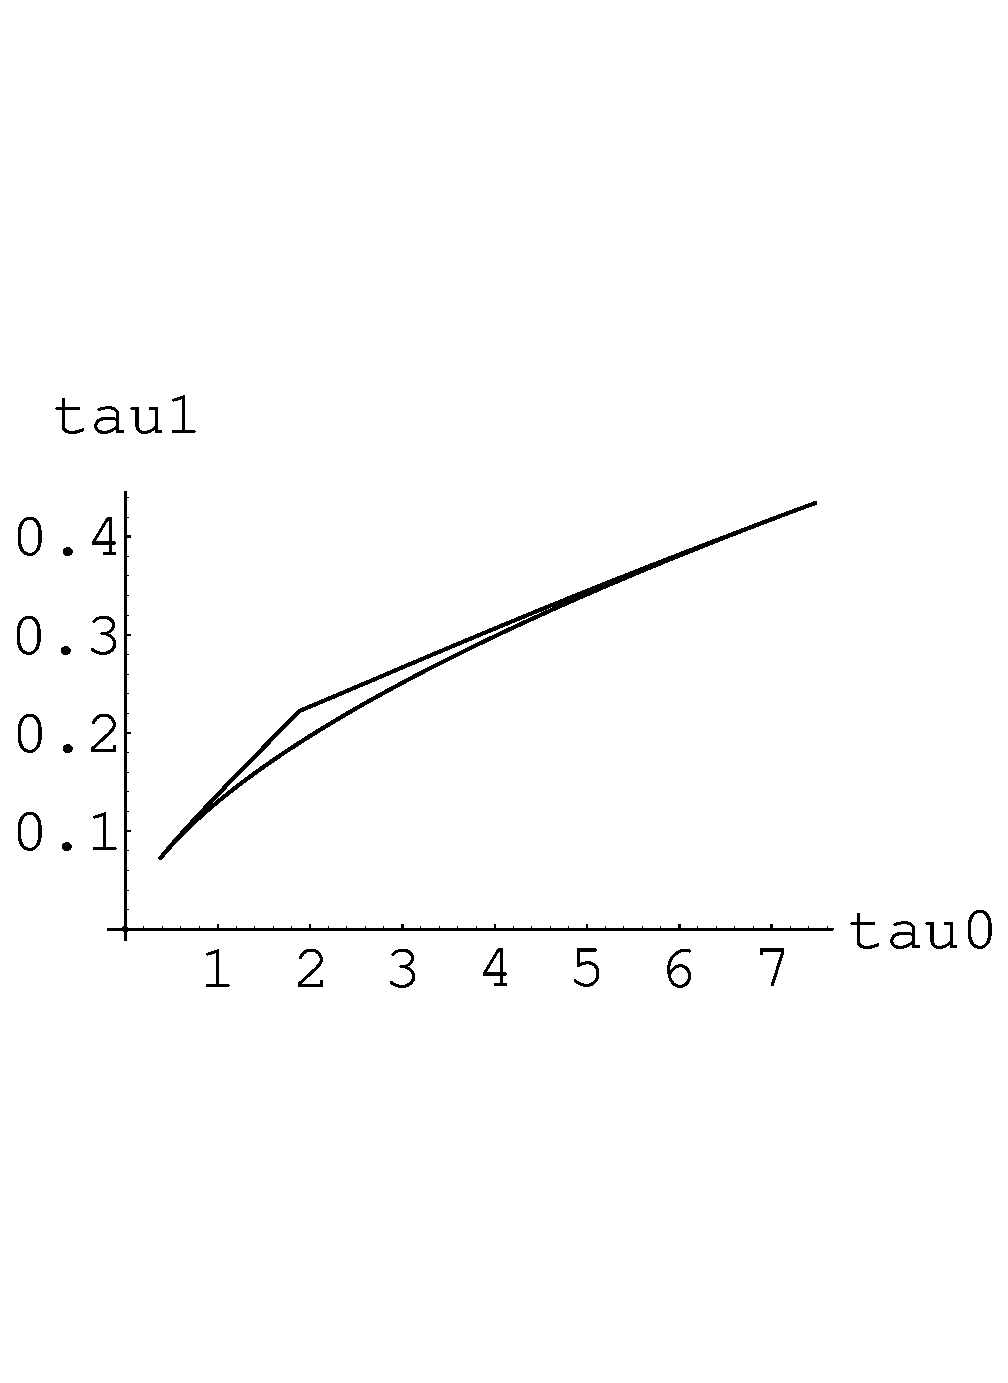
\epsfig{file=Figures/figure2.ps,height=5cm,bbllx=72pt,bblly=250pt,
bburx=540pt,bbury=540pt}
\caption{\label{f:taurange} The triangular region of the previous
figure is mapped into a distorted triangle in the $(\tau_0,\tau_1)$
plane.  Here $f_0$ is 120 Hz.}
\end{center}
\end{figure}

\clearpage
\subsection{Structure: {\tt struct Scope}}
\setcounter{equation}0
The set of templates is described by a structure {\tt struct Scope}.
This structure specifies a set of templates covering the mass range in
parameter space described above and shown in Figure \ref{f:taurange}.
The fields of this structure are:\\
\noindent
{\tt struct Scope} \{
\begin{description}
\item{\tt int n\_tmplt:}
    This integer is the total number of templates needed to cover the
    region in parameter space.  This is typically computed or set by
    {\tt template\_grid()}.
\item{\tt float m\_mn:}
   The minimum mass of an object in the binary system, as described above, in solar masses.
\item{\tt float m\_mx:}
   The maximum mass of an object in the binary system, as described
   above, in solar masses.  Together with the {\tt m\_mn}, this
   describes the region in parameter space covered by the set of
   templates.
\item{\tt float theta:}
    The angle to the axis of the constant ambiguity ellipse whose
    axis has diameter {\tt dp}. The angle is measured in radians
    counterclockwise from the $\tau_0$ axis.  The range is $\theta \in
    (-\pi/2,\pi/2)$.
\item{\tt float dp:}
   The diameter along the ellipse (in sec).  This is
   twice the radius $r_1$ given in Table~\ref{t:ellipse}.
   The angle $\theta$ is measured to this axis.
\item{\tt float dq:}
   The diameter along the ellipse (in sec).  This is
   twice the radius $r_2$ given in Table~\ref{t:ellipse}.
\item{\tt float f\_start:}
   The frequency $f_0$ used in the definitions of $\tau_0$ and $\tau_1$
   (\ref{e:tau0},\ref{e:tau1}); this is typically the frequency at
   which a binary chirp first enters the usable bandpass of the
   detector.
\item{\tt struct Template* templates:}
   Pointer to the array of templates.  This pointer is typically set by
   {\tt template\_grid()}, when it allocates the memory necessary to
   store the templates, and creates the necessary templates.
\end{description}
\};

Note that a given constant ambiguity ellipse can be specified in either of two
equivalent ways.  For example the elllipse
defined by
\begin{equation}
\theta = \pi/4, dp=1 {\rm \ msec}, dq=5 {\rm \ msec}
\end{equation}
is completely equivalent to the ellipse
\begin{equation}
\theta = 5 \pi/4, dp=5 {\rm \ msec}, dq=1 {\rm \ msec}.
\end{equation}
Either of these is acceptable.  The literature frequently uses the second convention (angle measured to the
major axis).

\clearpage
\subsection{Function: {\tt  tau\_of\_mass()}}
\label{ss:tau_of_mass}
\setcounter{equation}0
{\tt void tau\_of\_mass(double m1, double m2, double pf, double *tau0, double *tau1)}\\
This function calculates the coordinates $(\tau_0,\tau_1)$ associated
with particular values of the masses of the objects in the binary system, and a particular
value of frequency $f_0$.

The arguments are:
\begin{description}
\item{\tt m1}: Input.  The first mass (in solar masses).
\item{\tt m2}: Input.  The second mass (in solar masses).
\item{\tt pf}: Input.  The value $\pi f_0$. Here $f_0$ is the frequency
  used in defining the $\tau$ coordinates (see below).  It is often
  chosen to be at (or below) the frequency at which the chirp first
  enters the bandpass of the gravitational wave detector.
\item{\tt tau0}: Output.  Pointer to $\tau_0$ (in seconds).
\item{\tt tau1}: Output.  Pointer to $\tau_1$ (in seconds).
\end{description}

Although one can think of $\tau_0$ and $\tau_1$ as coordinates in the
parameter space defined by (\ref{e:tau0}) and (\ref{e:tau1}) they have
simple physical meanings.  $\tau_0$ is the time to coalescence of the
binary system, measured from the time that the waveform passes through
frequency $f_0$, in the zeroth post-Newtonian approximation.  $\tau_1$
is the first-order post-Newtonian correction to this quantity, so that
to this order the time to coalescence is $\tau_0+\tau_1$.
\begin{description}
\item{Author:}
Bruce Allen, ballen@dirac.phys.uwm.edu
\item{Comments:}
None.
\end{description}
\clearpage

\subsection{Function: {\tt m\_and\_eta()}}
\label{ss:m_and_eta}
\setcounter{equation}0
{\tt int m\_and\_eta(double tau0, double tau1, double *M, double *eta, double Mmin, double Mmax, double pf)}\\
This function takes as inputs the coordinates $(\tau_0,\tau_1)$.  If
these correspond to individual masses $m_1$ and $m_2$ each lying in the
range from $M_{\min}$ to $M_{\rm max}$ then the function sets the total
mass $M=m_1+m_2$ and sets $\eta = m_1 m_2/(m_1+m_2)^2$ and returns the
value 1.  Otherwise, the function returns 0 and does not change the
values of mass $M$ or $\eta$.

The arguments are:
\begin{description}
\item{\tt tau0} Input.  The value of $\tau_0$ (positive, sec).
\item{\tt tau1} Input.  The value of $\tau_1$ (positive, sec).
\item{\tt M} Output.  The total mass $M$ (solar masses).  Unaltered if
no physical mass values are found in the desired range.
\item{\tt eta} Output.  The value of $\eta$ (dimensionless).  Unaltered
if no physical mass values are found in the desired range.
\item{\tt Mmin} Input.  Minimum mass of one object in the binary pair,
  in solar masses (positive).
\item{\tt Mmax} Input.  Maximum mass of one object in the binary pair,
  in solar masses (positive).
\item{\tt pf}: Input.  The value $\pi f_0$. Here $f_0$ is the frequency at which
  the chirp first enters the bandpass of the gravitational wave detector.
\end{description}
The algorithm followed by {\tt m\_and\_eta()} is as follows.  Eliminate
$\eta$ from the equations defining $\tau_0$ (\ref{e:tau0}) and $\tau_1$
(\ref{e:tau1}) to obtain the following relation:
\begin{equation}
\label{e:rooteqn}
c_1 + c_2 \left( {M \over M_\odot} \right)^{5/3} - c_3 \left( {M \over M_\odot} \right) = 0,
\end{equation}
with the constants given by:
\begin{eqnarray}
\nonumber c_1 &=& 1155 \; T_\odot \\
c_2 &=& 47552 \; (\pi f_0 T_\odot )^{8/3} \tau_0\\
\nonumber c_3 &=& 16128 \; (\pi f_0 T_\odot )^2 \tau_1.
\end{eqnarray}
Given $(\tau_0,\tau_1)$ our goal is to find the roots of equation
(\ref{e:rooteqn}).  It is easy to see that the function on the lhs of
(\ref{e:rooteqn}) has at most two roots.  The function is positive at
$M=0$ but decreasing for small positive $M$.  However it is positive and
increasing again as $M \rightarrow \infty$.  Hence the function on the
lhs of (\ref{e:rooteqn}) has at most a single minimum for $M>0$.
Setting the derivative equal to zero and solving, this minimum lies at
a value of the total mass $M_{\rm crit}$ which satisfies
\begin{equation}
{M_{\rm crit} \over M_\odot} =
   \left( {3 \over 5} \; {c_3 \over c_2} \right)^{3/2}
\end{equation}
Hence the lhs of (\ref{e:rooteqn}) has no roots if its value is
positive at $M=M_{\rm crit}$ or it has two roots if that value is
negative.  (The ``set of measure zero" possibility is a single root at
$M_{\rm crit}$.)

If $2 M_{\rm min} < M_{\rm crit} < 2 M_{\rm max}$ then {\tt
m\_and\_eta()} searches for roots $2 M_{\rm min} < M < M_{\rm crit} $
and $  M_{\rm crit} < M< 2 M_{\rm max}$ separately, else it looks for a
root $M$ in the range $2 M_{\rm min} < M  < 2 M_{\rm max}$.  If
the lhs of (\ref{e:rooteqn}) changes sign at the upper and lower
boundaries of the interval, then a double-precision routine, similar to
the {\it Numerical Recipes} routine {\tt rtsafe()}, is used to obtain
the root with a combination of ``safe" bisection and ``rapid"
Newton-Raphson.

If a root $M$ is found in the desired range, then $\eta$ is
determined by (\ref{e:tau0}) to be
\begin{equation}
\eta={5 \over 256} \left( {M \over M_\odot} \right)^{-5/3}
(\pi f_0 T_\odot)^{-8/3} {T_\odot \over \tau_0}
\end{equation}
If $\eta \le
1/4$ then the smaller and larger masses are calculated from
\begin{equation}
m_1 = {M \over 2} \left(1-\sqrt{1-4\eta}\right) \quad
m_2 = {M \over 2} \left(1+\sqrt{1-4\eta}\right).
\end{equation}
(If both roots for $M$ correspond to $\eta \le 1/4$ then an error
message is generated and the routine aborts.) If both $m_1$ and $m_2$
are in the desired range $M_{\rm min} < m_1,m_2 <  M_{\rm max}$ then
{\tt m\_and\_eta()} returns 1 and sets $M$ and $\eta$ appropriately,
else it returns 0, leaving $M$ and $\eta$ unaffected.
\begin{description}
\item{Author:}
Bruce Allen, ballen@dirac.phys.uwm.edu
\item{Comments:}
Although the arguments to this function are double precision floats,
the values of $m_1$ and $m_2$ that may be inferred from them can
generally only be determined to single precision, particulary in the
neighborhood of $m_1=m_2$.  The reason is that in the vicinity of $\eta
\sim 1/4$, a fractional error $\epsilon$ is the value of $\eta$
produces a fractional error $\sqrt{\eta}$ in the masses.
\end{description}
\clearpage

\subsection{Function: {\tt template\_area()}}
\label{ss:area}
\setcounter{equation}0
{\tt float template\_area(struct Scope *Grid)}\\
This function computes
the area of the enclosed region of
parameter space shown in Figure \ref{f:taurange}.

The arguments are:
\begin{description}
\item{\tt Grid}: Input. This function uses only the minimum mass,
maximum mass and the cut-off frequency $f_0$ fields of {\tt Grid}.
\end{description}
The function returns the numerical value of the area in units of ${\rm
sec}^2$.  See the example in the following subsection.

The function uses an analytic expression for the area obtained by
integration of formulae (\ref{e:tau0},\ref{e:tau1}) for $\tau_0$
and $\tau_1$ given earlier.  For example, to obtain the area of the
trapezoidal region bounded above by the maximum-mass curve and below by
the $\tau_0$ axis, we integrate
\begin{eqnarray*}
A_{1} &=& \int_{m_{\rm max}}^{m_{\rm min}} 
\tau_1 (m_{\rm min},m) {d \tau_0(m_{\rm min},m) \over dm} dm\\
&=&
A_0 \left [ {m_{\rm min} \over M_{\odot} }\right ]^{8/3}
\biggl\{ 
{-[3 +2(4+2a)u + (5+9a)u^2 ] \over 2 u^2 (1+u)^{2/3} } \\
&+&{9a-1\over\sqrt{3} }\arctan \left [{1+2(1+u)^{1/3} \over \sqrt{3}} \right ]\\
&+& {9a-1\over 6 } \log\left [ 
{ 1 + (1+u)^{1/3} + (1+u)^{2/3}  \over  1 - 2 (1+u)^{1/3} + (1+u)^{2/3} } 
\right ]
\biggr\}_{u=m_{\rm min}/m_{\rm max}}^{u=1} \; .
\end{eqnarray*}
Here $a=924/743$ and $A_0$ is a quantity with dimensions ${\rm sec}^2$ 
given by 
\begin{eqnarray*}
A_0={18575 \over 49545216 }{ M_{\odot}^2 \over (\pi M_{\odot} f_0 )^{14/3} } 
\left ( {c^3 \over G } \right )^{8/3} \;.
\end{eqnarray*}

The area $A_{2}$ under the minimum-mass curve can be obtained from the
formula above by interchanging $m_{\rm min}$ and $m_{\rm max}$.  (If you wish
to use geomtrized units in which the solar mass is $4.92\times10^{-6}
\> {\rm sec}$ simply set $G=c=1$.) The area under the equal-mass curve
$A_{3}$ can be obtained by performing a similar integration along the
equal-mass curve
\begin{eqnarray*}
A_{3} &=& \int_{m_{\rm max}}^{m_{\rm min}} 
\tau_1 (m,m) {d \tau_0(m,m) \over dm} dm\\
&=&{60875 \over 2064384} 
{  M_{\odot}^2  \over (\pi f_0 M_{\odot})^{14/3} } 
\left [ \left (  {M_{\odot}\over m_{\rm min}} \right )^{8/3}
- \left ( {M_{\odot}\over m_{\rm max}} \right )^{8/3} \right ]
\left ( {c^3 \over G } \right )^{8/3} \;.
\end{eqnarray*}
These three results can be combined to give the total area
enclosed
\begin{equation}
\label{e:area}
A_{total} = A_{1} + A_{2} - A_{3} \;.
\end{equation}
Equation (\ref{e:area}) is the basis of {\tt template\_area()}; the next
example shows an application of this function.
\begin{description}
\item{Author:}
Alan Wiseman, agw@tapir.caltech.edu
\item{Comments:}
None.
\end{description}
\clearpage

\subsection{Example: {\tt area} program}
\setcounter{equation}0
This example uses the function {\tt template\_area()} described in the
previous section to compute the area of the specified parameter space.
The parameters specifying the region  are set: the minimum and maximum
mass in solar masses and the cut off frequency in seconds$^{-1}$.  The
numerical value of the area is returned and printed.
\lgrindfile{Includes/area.tex}

%%%%%%%%%%%%%%%%%%%%%%%%%%%%%%%%%%%%%%%%%%%%%%%%%%%%%%%%%%%%%%%%%%%%%%%
%%%%%%%%%  WHAT FOLLOWS IS THE RESPONSIBILITY OF SCOTT HUGHES %%%%%%%%%
%%%%%%%%%%%%%%%%%%%%%%%%%%%%%%%%%%%%%%%%%%%%%%%%%%%%%%%%%%%%%%%%%%%%%%%
\clearpage
\subsection{The match between two templates}
\par\noindent
\label{ss:match}
When one performs a search for a gravitational wave signal
in noisy instrumental data, one lays a grid of templates out
in parameter space.  For instance, if one uses $\tau_0$ and
$\tau_1$ [see Eqs.\ (\ref{e:tau0}) and (\ref{e:tau1})] as
parameter space coordinates, then one's templates can be
described as a set of points $(\tau_0^i,\tau_1^i)$ (with
$i$ ranging from 1 to the total number of templates).  One
requires these points to be spaced such that no more than some
{\it a priori}\/ fraction of SNR is lost due to the
discreteness of the template family.

Suppose one has decided that a set templates can lose no more
than $3\%$ SNR in a search.  This means that if some arbitrary
signal $b(t)$ is dropped onto the template grid, there must exist
a template, $a(t)$, such that
\begin{equation}
\label{e:match1}
\max_{t_0}\int_{-\infty}^{\infty} df {{\tilde b}(f){\tilde a}^*(f)
\over S_h(f)} e^{-2\pi ift_0} \ge 
.97 \left[\int_{-\infty}^{\infty} df
{|{\tilde b}(f)|^2\over S_h(f)}\right]^{1/2}
\left[\int_{-\infty}^{\infty} df
{|{\tilde a}(f)|^2\over S_h(f)}\right]^{1/2}
\end{equation}
(``$\max t_0$'' indicates the integral on the left hand side
is to be maximized over all possible values of $t_0$.)  The integral
on the left is the SNR obtained when the signal $b(t)$ is measured
using the Wiener optimal filter corresponding to the template $a(t)$.
The first integral on the right is the SNR obtained when $b(t)$ is
measured with the Wiener optimal filter corresponding to a template
$b(t)$; the second when the signal and template are both $a(t)$.
(The integrals on the right hand side, in other words, describe the
situation in which the template exactly matches the signal).  For
a detailed discussion of Wiener filtering, see Section
\ref{ss:wienerfilt}.

To simplify this discussion, let us introduce the following inner
product:
\begin{equation}
\label{e:definprod2}
\langle a,b\rangle_{t_0} \equiv
\int_{-\infty}^{\infty} df {{\tilde a}^*(f){\tilde b}(f)\over S_h(f)}
e^{-2\pi ift_0}.
\end{equation}
[Note: this inner product is not to be confused with the inner
product $(a,b)$ defined in Eq.~(\ref{e:definprod}).]  We will use
the convention that not including the $t_0$ subscript on the angle
bracket is equivalent to $t_0 = 0$.  Eq.~(\ref{e:match1}) can now
be rewritten
\begin{equation}
\max_{t_0}\quad\langle a,b\rangle_{t_0} \ge .97\sqrt{\langle a,a\rangle
\langle b,b\rangle}.
\end{equation}
This motivates the definition of the {\it match} between $a(t)$
and $b(t)$:
\begin{equation}
\mu \equiv \max_{t_0}{\langle a,b \rangle_{t_0}\over\sqrt{\langle a,a\rangle
\langle b,b\rangle}}.
\end{equation}
The match can be thought of as a distance measure between $a(t)$
and $b(t)$ (it is in fact one of the starting points for the metric
that Owen defines in \cite{Owen}).  One uses the match function as a
means of determining how one must space templates on the parameter space.
If one requires that no more than $3\%$ of possible SNR be lost due to
template discreteness, then one must require adjacent templates to have
a match $\mu = .97$.

The next few functions described in this manual are tools that can
be used for calculating the match function and understanding how it
varies over one's parameter space.

\clearpage
\subsection{Function: \tt{compute\_match()}}
\label{ss:compute_match}

{\tt 
float compute\_match(float m1, float m2, float ch0tilde[], float
		    ch90tilde[], float inverse\_distance\_scale, float
		    twice\_inv\_noise[], float flo, float s\_n0, float
		    s\_n90, int npoint, float srate, int err\_cd\_sprs,
		    int order)
}\\
This function computes and returns the match function between
a binary inspiral template that is stored in the arrays {\tt
ch0tilde[]} and {\tt ch90tilde} and the binary inspiral template
that corresponds to the binary system whose bodies have masses {\tt m1}
and {\tt m2}.

The two phases of the ``reference chirp'', {\tt ch0tilde[]} and
{\tt ch90tilde[]}, are assumed to have been precomputed and run
through the function {\tt orthonormalize()}.  (The parameters
{\tt s\_n0} and {\tt s\_n90} are assumed to have been found when
the reference chirp was {\tt orthonormalize}d.)  This allows
efficient computation of the match of many different templates with
the reference chirp.

The arguments to the function are:

\begin{description}
\item{{\tt m1:}} Input. Mass of body 1 in the template that is
cross-correlated with the reference chirp, solar masses.
\item{{\tt m2:}} Input. Mass of Body 2 in the template, solar masses.
\item{{\tt ch0tilde:}} Input. The FFT of the $0^\circ$-phase reference
chirp.
\item{{\tt ch90tilde:}} Input. The FFT of the $90^\circ$-phase
reference chirp.
\item{{\tt inverse\_distance\_scale:}} Input. The inverse distance
to the binary system, in $1/$Mpc.  Because the match is a normalized
correlation, this parameter isn't physically relevant: moving the
binary twice as far from the earth has no effect on the match.
However, it may be computationally convenient to scale the inner
products that go into the match defintion by some amount to prevent
numerical error.
\item{{\tt twice\_inv\_noise:}} Input. Twice the inverse noise
power spectrum, used for optimal filtering.  For a more detailed
description, see the routine {\tt find\_chirp()} (which is used
within {\tt compute\_match()}).
\item{{\tt flo:}} Input. The low-frequency cutoff to impose, in Hz.
Within the code, this is used as the starting frequency of the
templates; see {\tt make\_filters()}.
\item{{\tt s\_n0:}} Input. The normalization of {\tt ch0tilde[]},
found using {\tt orthonormalize()}.
\item{{\tt s\_n90:}} Input. The normalization of {\tt ch90tilde[]},
found using {\tt orthonormalize()}.  Note that only the ratio
{\tt s\_n0/s\_n90} is physically relevant, because the match is
normalized; if both {\tt s\_n0} and {\tt s\_n90} are multiplied by
some constant, the match is unaffected.
\item{{\tt npoint:}} Input. Defines the lengths of the various arrays:
{\tt ch0tilde[0..npoint-1]}, $\qquad \qquad$ {\tt ch90tilde[0..npoint-1]},
{\tt twice\_inverse\_noise[0..npoint/2]}.
\item{{\tt srate:}} Input. The sampling rate, in Hz.  Used to convert
between integer array time-domain subscripts and frequency subscripts.
For example this is the sample rate of the $0^\circ$- and
$90^\circ$-phase reference chirps, before they are FFT'd.
\item{{\tt err\_cd\_sprs:}} Input. The error suppression code to be
passed to the chirp generator; see {\tt chirp\_filters()}.
\item{{\tt order:}} Input. Twice the post-Newtonian order; {\it i.e.},
the power of $(v/c)$ used in the expansion.  See {\tt chirp\_filters()}.
\end{description}

\begin{description}
\item{Author:} Scott Hughes, hughes@tapir.caltech.edu
\end{description}

\clearpage
\subsection{Function: \tt{match\_parab()}}
\label{ss:match_parab}
{\tt
int match\_parab(float m1ref, float m2ref, float matchcont, int order, float srate, 
                float flo, float ftau, char *noisefile, float *semimajor, 
                float *semiminor, float *theta, float mcoef[])
}\\
This function attempts to find a parabolic fit to the match
function near a reference template with masses ({\tt m1ref,m2ref}).
It works in ($\tau_0,\tau_1$) coordinates, and can can use any noise
curve listed in {\tt detectors.dat} for its inner products when
computing the match.

Let the coordinates of the reference chirp be ($\tau_0^r,\tau_1^r$),
and define $x\equiv\tau_0-\tau_0^r$, $y\equiv\tau_1-\tau_1^r$.  Then,
the fit to the match is of the form
\begin{eqnarray}
\mu &=& 1 + a x^2 + 2b xy + c y^2\nonumber\\
    &=& 1+\pmatrix{x&y\cr}\cdot\pmatrix{a&b\cr b&c\cr}\cdot
	\pmatrix{x\cr y\cr}.
\end{eqnarray}
Written in the form on the second line, it is easy to show that,
if the match is in fact parabolic, it has surfaces of constant value
that are ellipses.  The (unnormalized) eigenvectors of this matrix
are given by
\begin{eqnarray}
{\vec v}_0 &=& \pmatrix{x\cr\cr y\cr} =
\pmatrix{{(a-c)/2b}+\sqrt{\left[(a-c)/2b\right]^2+1}\cr\cr1\cr}\nonumber\\
\nonumber\\
{\vec v}_1 &=& \pmatrix{x\cr\cr y\cr} =
\pmatrix{{(a-c)/2b}-\sqrt{\left[(a-c)/2b\right]^2+1}\cr\cr1\cr},
\end{eqnarray}
and the eigenvalues are
\begin{eqnarray}
\lambda_0 &=& {1\over2}(a+c)+\sqrt{{1\over4}(a-c)^2 + b^2}\nonumber\\
\lambda_1 &=& {1\over2}(a+c)-\sqrt{{1\over4}(a-c)^2 + b^2}.
\end{eqnarray}
(Note: because the match is maximal at $x=y=0$ and falls off as $x$
and $y$ increase, the matrix is negative definite.  The eigenvalues
are therefore negative, and so $|\lambda_1| > |\lambda_0|$.)  From
these values, it is simple to construct the equimatch ellipse.
If the value of the match on the contour is $\mu_{\rm cont}$, then
the semimajor axis of the ellipse has length
\begin{equation}
r_{\rm major} = \sqrt{\mu_{\rm cont}-1\over\lambda_0},
\end{equation}
and the semiminor axis has length
\begin{equation}
r_{\rm minor} = \sqrt{\mu_{\rm cont}-1\over\lambda_1}.
\end{equation}
The counterclockwise angle between the semimajor axis and
the $\tau_0$ axis is easily found from ${\vec v}_0$:
\begin{equation}
\theta = {\tt atan2}(v_{0y},v_{0x}) =
\arctan\left({1/\left[{(a-c)/2b}+
\sqrt{\left[(a-c)/2b\right]^2+1}\right]}\right).
\end{equation}
(Here, {\tt atan2()} is the {\tt C} math library function; using
{\tt atan2()} insures that the computer points 
$\theta$ to the
correct quadrant of the $\tau_0,\tau_1$ plane.)
If we now define normalized eigenvectors ${\vec e}_0 =
{\vec v}_0/|{\vec v}_0|$,
${\vec e}_1 = {\vec v}_1/|{\vec v}_1|$, the ellipses are then
easily constructed using the parametric curve
\begin{equation}
\pmatrix{x\cr y} = r_{\rm major}\cos\phi\;{\vec e}_0 +
	r_{\rm minor}\sin\phi\;{\vec e}_1,
\end{equation}
with
$\phi$ varying from 0 to $2\pi$.

The arguments to the function are:

\begin{description}
\item{\tt{m1ref}}: Input.  Mass of body 1 for the reference chirp
(solar masses).
\item{\tt{m2ref}}: Input.  Mass of body 2 for the reference chirp
(solar masses).
\item{\tt{matchcont}}: Input.  The value of the match contour.
\item{\tt{order}}: Input.  Twice the post-Newtonian order to be
used in computing the templates; {\it i.e.}, the power of $(v/c)$
used in the post-Newtonian expansion.
\item{\tt{srate}}: Input.  The sample rate, in Hz.  Used to convert
between integer array time-domain subscripts and frequency subscripts.
For example this is the sample rate of the $0^\circ$- and
$90^\circ$-phase reference chirps, before they are FFT'd.
\item{\tt{flo}}: Input. The low-frequency cutoff to impose, in
Hz. Within the code, this is used as the starting frequency of
the templates; see {\tt make\_filters()}.
\item{\tt{ftau}}: Input. The frequency used to find $\tau_0$
and $\tau_1$; see Eqs.\ (\ref{e:tau0}) and (\ref{e:tau1}).
Different authors use different conventions for this
frequency---for example, Sathyaprakash uses the seismic wall
frequency, whereas Owen uses the frequency at which the noise
power is minimum.  {\tt ftau} is arbitrary, but should be used
consistently: pick a value and stick with it.
\item{\tt{noisefile}}: Input.  A character string that specifies
the name of a data file containing information about the noise
power spectrum $P(f)$ of a dectector.  See {\tt noise\_power()}
for extended discussion.
\item{\tt{semimajor}}: Output.  The semimajor axis of the ellipse
along which the match has the value {\tt matchcont}.
\item{\tt{semiminor}}: Output.  The semiminor axis of the ellipse.
\item{\tt{theta}}: Output.  The counterclockwise angle, in radians,
between {\tt semimajor} and the $\tau_0$ axis.
\item{\tt{mcoef}}: Output.  The array {\tt mcoef[0..2]} contains the
coefficients of the parabolic fit to the match:
$\mu_{\rm fit} = 1 + {\hbox{\tt mcoef[0]}} x^2 + {\hbox{\tt mcoef[1]}} xy +
{\hbox{\tt mcoef[2]}} y^2$.
\end{description}

The function works by sampling many templates in ($\tau_0,\tau_1$)
coordinates that are close to the template with masses
({\tt m1ref,m2ref}).  Periodically, it computes the best parabolic fit
to the data it has gathered so far and constructs the elliptical
contour corresponding to that fit.  It then takes $N_{\rm ell}$ steps
around this ellipse and compares the value of the match predicted
by the fit with the actual match value at each point.  It then computes
the following ``$\chi^2$-like'' statistic:
\begin{equation}
\varepsilon = {1\over N_{\rm ell}}\sum_{i=1}^{N_{\rm ell}}
\left(\mu_{\rm actual}^i - \mu_{\rm fit}^i\over 10^{-3}\right)^2.
\end{equation}
If $\varepsilon=1$, then each fit point differs from the match by
$10^{-3}$.  A ``good'' fit will have $\varepsilon$ of order 1.

This function returns 0 if a good fit is not found ($\varepsilon$
is greater than 5 yet more than 250 templates have been
used to generate fit data), and 1 otherwise.  If a good fit is
not found, then the match is not parabolic in the vicinity of the
template ({\tt m1ref,m2ref}) down to $\mu={\tt matchcont}$.  This
is typically the case if the masses are large (so that there are
few cycles measured, and relativistic effects are very important),
and if the value of {\tt matchcont} is too far from 1.  For instance,
with the LIGO 40-meter prototype, {\tt match\_parab()} cannot
find a parabolic fit to the .97 match contour for a binary with
$m_1 = 1.2 M_\odot$, $m_2 = 1.6 M_\odot$; but it {\it does} find
a parabolic fit for this binary at the .99 match contour.

\begin{description}
\item{Author:} Scott Hughes, hughes@tapir.caltech.edu
\end{description}

\clearpage
\subsection{Function: \tt{match\_cubic()}}
\label{ss:match_cubic}

{\tt
int match\_cubic(float m1ref, float m2ref, float matchcont, int order, float srate, 
                float flo, float ftau, char *noisefile, float *semimajor, 
                float *semiminor, float *theta, float mcoef[])
}\\
This function is almost identical to {\tt match\_parab()}, except
that it attempts to fit the match to a cubic form:

\begin{equation}
m = 1 + a x^2 + 2b xy + c y^2 + dx^3 + e y^3 + fx^2y + g xy^2
\end{equation}

The arguments to the function are:

\begin{description}
\item{\tt{m1ref}}: Input.  Mass of body 1 for the reference chirp
(solar masses).
\item{\tt{m2ref}}: Input.  Mass of body 2 for the reference chirp
(solar masses).
\item{\tt{matchcont}}: Input.  The value of the match contour.
\item{\tt{order}}: Input.  Twice the post-Newtonian order to be
used in computing the templates; {\it i.e.}, the power of $(v/c)$
used in the post-Newtonian expansion.
\item{\tt{srate}}: Input.  The sample rate, in Hz.  Used to
determine the spacing of frequency bins for the templates.
\item{\tt{flo}}: Input. The low-frequency cutoff to impose, in
Hz. Within the code, this is used as the starting frequency of
the templates; see {\tt make\_filters()}.
\item{\tt{ftau}}: Input. The frequency used to find $\tau_0$
and $\tau_1$; see Eqs.\ (\ref{e:tau0}) and (\ref{e:tau1}).
Different authors use different conventions for this
frequency---for example, Sathyaprakash uses the seismic wall
frequency, whereas Owen uses the frequency at which the noise
power is minimum.  {\tt ftau} is arbitrary, but should be used
consistently: pick a value and stick with it.
\item{\tt{noisefile}}: Input.  A character string that specifies
the name of a data file containing information about the noise
power spectrum $P(f)$ of a dectector.  See {\tt noise\_power()}
for extended discussion.
\item{\tt{semimajor}}: Output.  The semimajor axis of the ellipse
along which the match has the value {\tt matchcont}.
\item{\tt{semiminor}}: Output.  The semiminor axis of the ellipse.
\item{\tt{theta}}: Output.  The counterclockwise angle, in radians,
between {\tt semimajor} and the $\tau_0$ axis.
\item{\tt{mcoef}}: Output.  The array {\tt mcoef[0..6]} contains the
coefficients of the parabolic fit to the match:
$\mu_{\rm fit} = 1 + {\hbox{\tt mcoef[0]}} x^2 + {\hbox{\tt mcoef[1]}} xy +
{\hbox{\tt mcoef[2]}} y^2 + {\hbox{\tt mcoef[3]}} x^3 +
{\hbox{\tt mcoef[4]}} y^3 + {\hbox{\tt mcoef[5]}} x^2y +
{\hbox{\tt mcoef[6]}} xy^2$.
\end{description}

The function works in almost exactly the same manner as {\tt
match\_parab()}.  In particular, it constructs an ellipse using
the parabolic piece of the cubic fit, and checks the goodness
of the fit along that ellipse.  Because the ellipse is not made
from the full functional form of the fit, the fit does not have
constant value along the ellipse.  Thus, {\tt match\_cubic()}
does not really find contours with constant match value
{\tt matchcont}.  The ellipses it finds, however, generally
have match values fairly close to {\tt matchcont}; and, more
importantly, the match values along the ellipse are never less
than {\tt matchcont}.

\begin{description}
\item{Author:} Scott Hughes, hughes@tapir.caltech.edu
\end{description}

\clearpage
\subsection{Example: {\tt match\_fit} program}
\label{ss:match_fit}

This program will try to find the fit to the match function
about some template.  It is called with four arguments: the
mass of body 1 (in solar masses), the mass of body 2 (in
solar masses), the value of the match for which it tries
to fit, and (twice) the order of the post-Newtonian expansion
used to compute the templates.  For example,
{\tt match\_fit 1.2 1.8 .98 4} will try to find a fit to
the .98 match contour near the template for the
$1.2\,M_\odot-1.8\,M_\odot$ using post-2-Newtonian templates.

The program first attempts to find a parabolic fit; if it
is unable to do so, it then tries a cubic.  If the cubic
fails, you are in a region of parameter space where the match
is badly behaved.  This is typically the case if you ask for
masses that are too large---for example, no fit can be found
near a $5\,M_\odot-5\,M_\odot$ solar mass binary with the
LIGO 40-meter prototype noise curve.  When the masses are large,
the system radiates very few gravitational-wave cycles in the
instrument's frequency band; and, those cycles typically correspond
to a strongly relativistic regime of inspiral.  If you find
yourself in this circumstance, either give up on the large
mass binaries, or try to find a fit at a match level closer to
1.

\lgrindfile{Includes/match_fit.tex}

\begin{description}
\item{Author:} Scott Hughes, hughes@tapir.caltech.edu
\end{description}



%%%%%%%%%%%%%%%%%%%%%%%%%%%%%%%%%%%%%%%%%%%%%%%%%%%%%%%%%%%%%%%%%%%%%%%
%%%%%%%%%       END OF RESPONSIBILITY OF SCOTT HUGHES         %%%%%%%%%
%%%%%%%%%%%%%%%%%%%%%%%%%%%%%%%%%%%%%%%%%%%%%%%%%%%%%%%%%%%%%%%%%%%%%%%

%%%%%%%%%%%%%%%%%%%%%%%%%%%%%%%%%%%%%%%%%%%%%%%%%%%%%%%%%%%%%%%%%%%%%%
%%%%%%%%   BEGINNING OF RESPONSIBILITY OF TEVIET CREIGHTON   %%%%%%%%%
%%%%%%%%%%%%%%%%%%%%%%%%%%%%%%%%%%%%%%%%%%%%%%%%%%%%%%%%%%%%%%%%%%%%%%

\clearpage
\subsection{Structure: {\tt struct cubic\_grid}}
\label{ss:cubic_grid}

This structure is used to store precomputed coefficients of the cubic
fit to the match function, generated by {\tt match\_cubic()} on an
equally spaced grid in the $m_1,m_2$ parameter space.  The stucture
stores the coefficients as well as all the information required to
generate, retrieve, and interpolate among them.  The fields of this
structure are:

\noindent{\tt struct cubic\_grid} \{
\begin{description}
\item{\tt int n;}
  The number of points along the side of the grid.

\item{\tt float m\_mn;}
  The minimum mass of an object in the parameter space covered by the
  grid (solar masses).

\item{\tt float m\_mx;}
  The minimum mass of an object in the parameter space covered by the
  grid (solar masses).

\item{\tt float dm;}
  The spacing between grid points (solar masses); equal to $(\hbox{\tt
  m\_mx}-\hbox{\tt m\_mn})/(\hbox{\tt n}-1)$.

\item{\tt float match;}
  The match level (between 0 and 1) out to which the cubic fit was
  made.

\item{\tt float angle;}
  The angle (radians) counterclockwise from the $\tau_0$ axis to the
  $x$ axis (see below).

\item{\tt int order;}
  Twice the post-Newtonian order of the chirp templates used to
  compute the match function.

\item{\tt float srate;}
  The sampling rate of the chirp templates used to compute the match
  function.

\item{\tt float flo;}
  The initial frequency of the chirp templates used to compute the
  match function.

\item{\tt float ftau;}
  The reference frequency used to define the $\tau_0,\tau_1$
  coordinates.

\item{\tt int detector;}
  The index of the detector site in the data file {\tt detectors.dat},
  used to identify a noise curve for computing the match function.

\item{\tt float ***coef;}
  A pointer to the array of coefficients.

\end{description}
\};

The {\tt cubic\_grid.coef} field points to an array of the form {\tt
coef[0..n-1][0..n-1][0..9]}.  The first two indecies {\tt [i][j]}
identify a point in the mass parameter space: $m_1=\hbox{\tt
m\_mn}+\hbox{\tt i}\times\hbox{\tt dm}$ and $m_2=\hbox{\tt
m\_mn}+\hbox{\tt j}\times\hbox{\tt dm}$.  The third index identifies a
particular coefficient computed at that point.  The individual
coefficients are defined as follows: The first 7 entries {\tt [0..6]}
are the actual coefficients of the cubic fit to the match function
$\mu$:
\begin{equation}
\label{e:cubicmatch}
	\mu = 1 + {\hbox{\tt [0]}}x^2 + {\hbox{\tt [1]}}xy
		+ {\hbox{\tt [2]}}y^2 + {\hbox{\tt [3]}}x^3
		+ {\hbox{\tt [4]}}y^3 +	{\hbox{\tt [5]}}x^2y
		+ {\hbox{\tt [6]}}xy^2 \; ,
\end{equation}
where $x,y$ are small displacements in directions at an angle {\tt
cubic\_grid.angle} counterclockwise from the $\tau_0,\tau_1$
directions, respectively.  If one considers only the quadratic part of
this fit, the equation $\mu=\hbox{\tt cubic\_grid.match}$ defines an
ellipse in the $x,y$ plane.  Entries {\tt [7]} and {\tt [8]} are then
the semimajor and semiminor axes of this ellipse, respectively (in
units of seconds), and entry {\tt [9]} is the angle (in radians)
counterclockwise from the $x$ axis to the semimajor axis.  The entries
{\tt [7..9]} can be computed without too much difficulty from the
entries {\tt [0..2]} and the value of {\tt match}, but it can be
useful to have them precomputed.


\clearpage
\subsection{Function: {\tt generate\_cubic}}
\label{ss:generate_cubic}

\begin{verbatim}
void generate_cubic(struct cubic_grid grid, char *detectors_file,
                    const char *outfile, const char *logfile);
\end{verbatim}
This routine computes the coefficients of the cubic fit to the match
function on a mesh in parameter space, and writes the results to an
ASCII textfile, suitable for reading by the routine {\tt
read\_cubic()} (section~\ref{ss:read_cubic}).

The arguments are:

\begin{description}
\item{\tt grid:}
  Input/Output.  This structure contains the parameters for the
  computation of the cubic fits.  All of the fields except for {\tt
  grid.dm} and {\tt grid.coef} must be set; those fields are the ones
  that are computed.

\item{\tt detectors\_file:}
  Input.  The name of a data file containing detector site
  information, such as detectors.dat.  This is used to get a noise
  file for computing the match function.

\item{\tt outfile:}
  Input.  The name of the output file to which the coefficients and
  related information will be written.

\item{\tt logfile:}
  Input.  The name of a log file which tracks the progress of this
  routine (since it can take several hours to generate a reasonable
  grid).

\end{description}

The output file is an ASCII textfile containing the fields of the
structure {\tt grid}.  Each field except the {\tt coef} field is
printed on a separate line of the output file.  The {\tt coef} data is
written as $0.5\times\hbox{\tt grid.n}\times(\hbox{\tt grid.n}+1)$
lines of 10 floating point numbers; each line represents the 10
coefficients {\tt coef[i][j][0..9]} for a given {\tt i,j}.  The lines
are ordered by increasing {\tt j} from 0 to {\tt i} for each {\tt i}
from 0 to {\tt grid.n}-1.  Integers are printed exactly; floats are
printed in 10-digit precision exponential notation.

One should also note that this routine can take quite a long time to
run: on a 100~MHz pentium it typically takes 10 to 15 minutes per
point in the grid.  This is the reason for creating the log file to
track the routine's progress.

\begin{description}
\item{Author:}
  Teviet Creighton, teviet@tapir.caltech.edu
\end{description}


\clearpage
\subsection{Function: {\tt regenerate\_cubic}}
\label{ss:regenerate_cubic}

\begin{verbatim}
int regenerate_cubic(char *detectors_file, const char *infile,
                     const char *outfile, const char *logfile);
\end{verbatim}
It may happen that the routine {\tt generate\_cubic()} terminates
before completing the entire coefficient grid.  Since each grid point
takes so long to compute, it would be foolish to discard those already
generated.  This routine, therefore, reads in a partially-complete
data file, and then continues the computation where {\tt
generate\_cubic()} left off.  The results are written to a new data
file (leaving the original file incomplete).  It returns 0 upon
successful completion, or 1 if the data file was absent or corrupt.
{\tt regenerate\_cubic()} also creates its own log file to track its
progress.

The arguments are:

\begin{description}
\item{\tt detectors\_file:}
  Input.  The name of a data file containing detector site
  information, such as {\tt detectors.dat}.  This is used to get a
  noise file for computing the match function.

\item{\tt infile:}
  Input.  The name of the incomplete data file of coefficients.

\item{\tt outfile:}
  Input.  The name of the data file where this routine stores its
  results.

\item{\tt logfile:}
  Input.  The name of a log file which tracks the progress of this
  routine.

\end{description}

\begin{description}
\item{Author:}
  Teviet Creighton, teviet@tapir.caltech.edu
\end{description}


\clearpage
\subsection{Function: {\tt read\_cubic}}
\label{ss:read_cubic}

\begin{verbatim}
int read_cubic(struct cubic_grid *grid, char *infile);
\end{verbatim}
This routine reads a textfile generated by {\tt generate\_cubic()},
stores the data in a variable {\tt grid} of type {\tt struct
cubic\_grid}, and passes this structure back.  {\tt read\_cubic()}
itself returns 0 after successful completion, or 1 if the data file
was absent or corrupt (in which case {\tt grid} is left unchanged).

Note that memory for the coefficient array grid.coef is allocated in
this routine; to free this memory, call {\tt free\_cubic(grid)}.
Allocating and de-allocating this array requires some care: since {\tt
grid.coef[i][j][k]} is necessarily symmetric in the first two
indecies, the pointers {\tt grid.coef[i][j]} and {\tt grid.coef[j][i]}
have been explicitly set to point to the same memory location, in
order to save memory.

The arguments are:

\begin{description}
\item{\tt grid:}
  Output.  The coefficient array and related data read from the data
  file.

\item{\tt infile:}
  Input.  The name of the data file.

\end{description}

\begin{description}
\item{Author:}
  Teviet Creighton, teviet@tapir.caltech.edu
\end{description}


\clearpage
\subsection{Function: {\tt get\_cubic}}
\label{ss:get_cubic}

\begin{verbatim}
int get_cubic(float m1, float m2, struct cubic_grid grid, float *coef);
\end{verbatim}
This routine computes the coefficients of a cubic fit to the match
function at a specified point in parameter space, by linear
interpolation of precomputed coefficients on a grid in parameter
space.  It returns 0 if successfully executed, or 1 if the point ({\tt
m1},{\tt m2}) lies outside of the grid.  In the latter case, {\tt
get\_cubic()} will compute extrapolated coefficients, but these are
unreliable.

The arguments are:

\begin{description}
\item{\tt m1:}
  Input.  One of the binary mass coordinates of the requested point in
  parameter space.

\item{\tt m2:}
  Input.  The other binary mass coordinates of the requested point in
  parameter space.

\item{\tt grid:}
  Input.  The data structure containing the precomputed coefficients
  and the information required to retrieve them.

\item{\tt coef:}
  Output.  The array {\tt coef[0..9]} is filled with the interpolated
  coefficients.

\end{description}

\begin{description}
\item{Author:}
  Teviet Creighton, teviet@tapir.caltech.edu
\end{description}


\clearpage
\subsection{Function: {\tt free\_cubic}}
\label{ss:free_cubic}

\begin{verbatim}
void free_cubic(struct cubic_grid grid);
\end{verbatim}
Frees the memory allocated to the array {\tt grid.coef} by {\tt
read\_cubic()}.

The argument is:

\begin{description}
\item{\tt grid:}
  Input.  The {\tt cubic\_grid} structure whose coefficient array is
  to be freed.

\end{description}

\begin{description}
\item{Author:}
  Teviet Creighton, teviet@tapir.caltech.edu
\end{description}


\clearpage
\subsection{Function: {\tt transform\_cubic}}
\label{ss:transform_cubic}

\begin{verbatim}
void transform_cubic(struct cubic_grid *grid, float angle, float match);
\end{verbatim}
This routine applies a rotation to the coefficients stored in {\tt
*grid}, and rescales the equimatch ellipses to a new match level.

The arguments are:

\begin{description}
\item{\tt grid:}
  Input/Output.  The structure containing the coefficients to be
  transformed.

\item{\tt angle:}
  Input.  The new value of {\tt grid.angle} (the elements {\tt
  (*grid).coef[i][j][0..6,9]} will be transformed to fit this new
  angle).

\item{\tt match:}
  Input.  The new value of {\tt grid.match} (the elements {\tt
  (*grid).coef[i][j][7,8]} will be rescaled according to this value).

\end{description}

\begin{description}
\item{Author:}
  Teviet Creighton, teviet@tapir.caltech.edu
\item{Comments:}
  The result of this transformation is not quite the same as if the
  grid were originally generated with the new value of the match.
  During initial generation of the grid, the match field also
  specifies the domain over which the cubic fit is made, as well as
  setting the scale for the equimatch ellipse axes.  This routine only
  rescales the ellipses; it does not regenerate a cubic fit over a new
  match range.
\end{description}


\clearpage
\subsection{Example: {\tt make\_grid} program}
\label{ss:make_grid}

This example program uses the function {\tt generate\_cubic()} to
create a grid of match function coefficients over the mass range of
0.8 to 3.2 solar masses, down to a match level of 0.98, using the
smooth fit to the LIGO noise power spectrum in computing the match
function.  The resulting grid structure is stored in the data file
{\tt cubic\_coef\_40meter\_m=0.8-3.2.ascii}.  Note that the program
can take quite a long time to run: approximately 20~hours on a 100~MHz
Pentium computer.  The program's progress is tracked in the log file
{\tt cubic\_coef\_40meter\_m=0.8-3.2.log}.

The program makes frequent calls to the routine {\tt match\_cubic()},
which generates a lot of messages in {\tt stderr}, which are generally
unimportant unless things go wrong.  You'll probably want to redirect
{\tt stderr} to some junk file.  The important progress record is
stored in {\tt cubic\_coef\_40meter\_m=0.8-3.2.log}, which, when
complete, looks like this:

\begin{verbatim}
Using Caltech-40 noise curve from the file noise_40smooth.dat.
Generating match coefficients at 91 points:
.
..
...
....
.....
......
.......
........
.........
..........
...........
............
.............

\end{verbatim}

The source code for {\tt make\_grid.c} is listed below:

\lgrindfile{Includes/make_grid.tex}

\begin{description}
\item{Author:}
  Teviet Creighton, teviet@tapir.caltech.edu
\end{description}


\clearpage
\subsection{Example: {\tt read\_grid} program}
\label{ss:read_grid}

This example program uses the function {\tt read\_cubic()} to read the
data file {\tt cubic\_coef\_40meter\_m=0.8-3.2.ascii} generated by
{\tt make\_grid} (section~\ref{ss:make_grid}), and return the
coefficients of the cubic fit to the match function for any point
$m_1,m_2$ in mass space.  Here are some sample runs of {\tt
read\_cubic}:

\begin{verbatim}
% read_grid 
Usage: read_grid M1 M2
% read_grid 1.3 1.5
Match coefficients: -5.075e+03  2.977e+04 -4.602e+04
                    -2.703e+04  6.656e+06  7.090e+05 -4.044e+06
Axis lengths:        9.245e-03  6.272e-04
Axis angle:          3.144e-01
% read_grid 1.3 3.5
(1.300,3.500) lies outside of grid.  Extrapolating...
Match coefficients: -4.159e+03  2.058e+04 -2.716e+04
                     2.866e+04  2.770e+06  1.424e+05 -1.620e+06
Axis lengths:        9.631e-03  8.116e-04
Axis angle:          3.688e-01
% 
\end{verbatim}

Masses are entered in solar masses.  However, the coefficients are the
cubic fit coefficients in $\tau_0,\tau_1$ space, so the first three
coefficients have units of s$^{-2}$, the next four coefficients of
s$^{-3}$, and the axis lengths of s.  The angle (counterclockwise from
the $\tau_0$ axis to the principle axis of the equimatch ellipse) is
in radians.

\lgrindfile{Includes/make_grid.tex}

\begin{description}
\item{Author:}
  Teviet Creighton, teviet@tapir.caltech.edu
\end{description}

%%%%%%%%%%%%%%%%%%%%%%%%%%%%%%%%%%%%%%%%%%%%%%%%%%%%%%%%%%%%%%%%%%%%%%
%%%%%%%%      END OF RESPONSIBILITY OF TEVIET CREIGHTON      %%%%%%%%%
%%%%%%%%%%%%%%%%%%%%%%%%%%%%%%%%%%%%%%%%%%%%%%%%%%%%%%%%%%%%%%%%%%%%%%


\clearpage
\subsection{Function: {\tt template\_grid()}}
\setcounter{equation}0
{\tt void template\_grid(struct Scope *Grid)}\\
This function evolved from {\tt grid4.f}, a FORTRAN routine written by
Sathyaprakash.  This function lays down a grid of templates
that cover a particular mass range (the region inside the distorted
triangle shown in Figure \ref{f:taurange}).

The arguments are:
\begin{description}
\item{\tt Grid}: Input/Output.
This function uses as input all of the fields of {\tt Grid} except for
{\tt Grid.n\_tmplt} and {\tt Grid.templates}.  On return from {\tt
template\_grid} these latter two fields are set.  The function uses
{\tt malloc()} to allocate storage space and creates in this space an
array containing {\tt Grid.n\_tmplt} objects of type {\tt Template}.
If you wish to free the memory, call {\tt free(Grid.templates)}.
\end{description}


It is easy to cover the parameter space shown in Figure
\ref{f:taurange} with ellipses.  However each ellipse represents a
filter, and filtering takes computer time and memory, so the real
problem is to cover the parameter space completely, using the {\it
smallest possible number} of templates.  This is a non-trivial {\it packing
problem}; while our solution is certainly not optimal, it is quite
close.

The algorithm used to place the templates works in coordinates
$(x_0,x_1)$ which are rotated versions of $(\tau_0,\tau_1)$, aligned
along the minor and major (or major and minor) axes of the template
ellipses.  The input angle {\tt Grid.theta},in the range $(-\pi,\pi)$,
is the counterclockwise angle through which the $(x_0,x_1)$ axes need
to be rotated to bring them into alignment with the principal axis of
the template ellipses.

Although each template is an ellipse, the problem of packing templates
onto the parameter space can be more easily described in terms of a more
familiar packing problem: packing pennies on the plane.  One can always
transform an ellipse into a circle by merely scaling one coordinate
uniformly while leaving the other coordinate unchanged.  So we
introduce coordinates $x_1$ along the major diameter and $x_o$ along
the minor diameter of the ellipse, and then ``shrinking" the $x_1$
coordinate by the ratio of major to minor diameters.  In this
way the ellipses are transformed into circles.

\begin{figure}[h]
\begin{center}
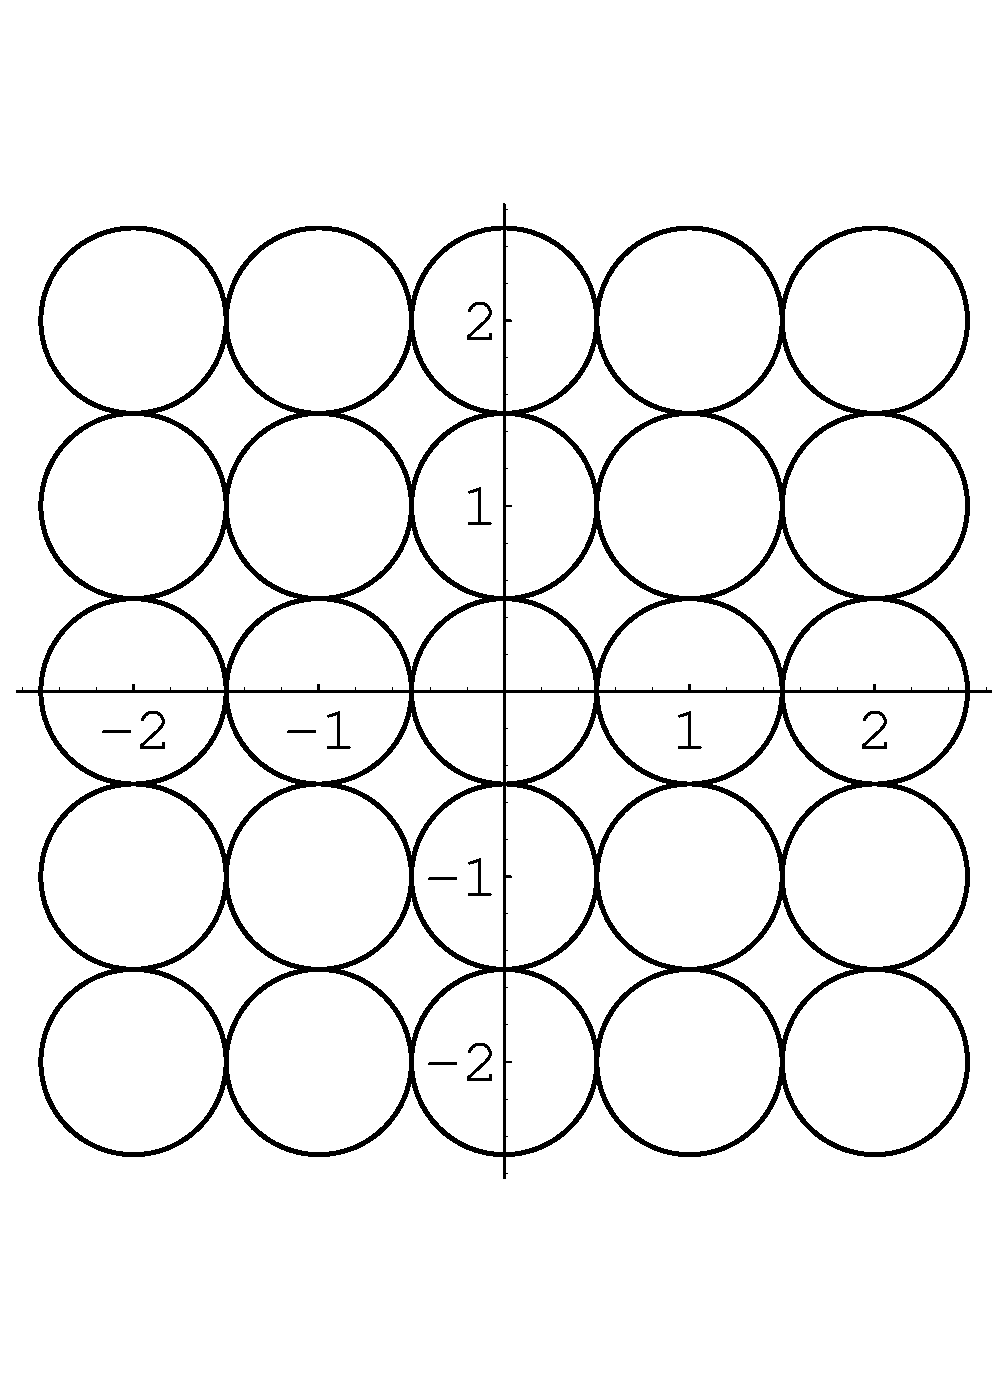
\epsfig{file=Figures/figure3.ps,height=4cm,bbllx=72pt,bblly=160pt,
bburx=540pt,bbury=630pt}
\caption{\label{f:pennies} Covering a plane with a square lattice of
pennies (or templates) leaves 21\% of the area exposed}
\end{center}
\end{figure}

First, a template is laid down at the point where the equal mass line
intersects the maximum mass line.  Then additional templates are placed
along the equal mass line, at increasing values of $x_0$.  These
templates are staggered up and down in the $x_1$ direction.  After
laying down this set of templates, the remaining part of parameter
space is covered with additional templates, in columns starting at each
of the previously determined template locations.  These columns have
the same value of $x_0$ as the previously determined templates but
increasing values of $x_1$.  The columns are continued until the
``leading edge" of the final template lies outside the parameter
space.

We can describe the packing (and the ``efficiency") of the packing in
terms of the penny-packing problem.  Suppose we start by setting
pennies of radius $1/2$ on all points in the plane with integer
coordinates, as shown in Figure \ref{f:pennies}.  It is easy to show
that the fraction of the plane (i.e., parameter space!) which is not
covered by any pennies is $\epsilon = 1-\pi/4 =0.214\cdots$ or about
21\%.
 
\begin{figure}[h]
\begin{center}
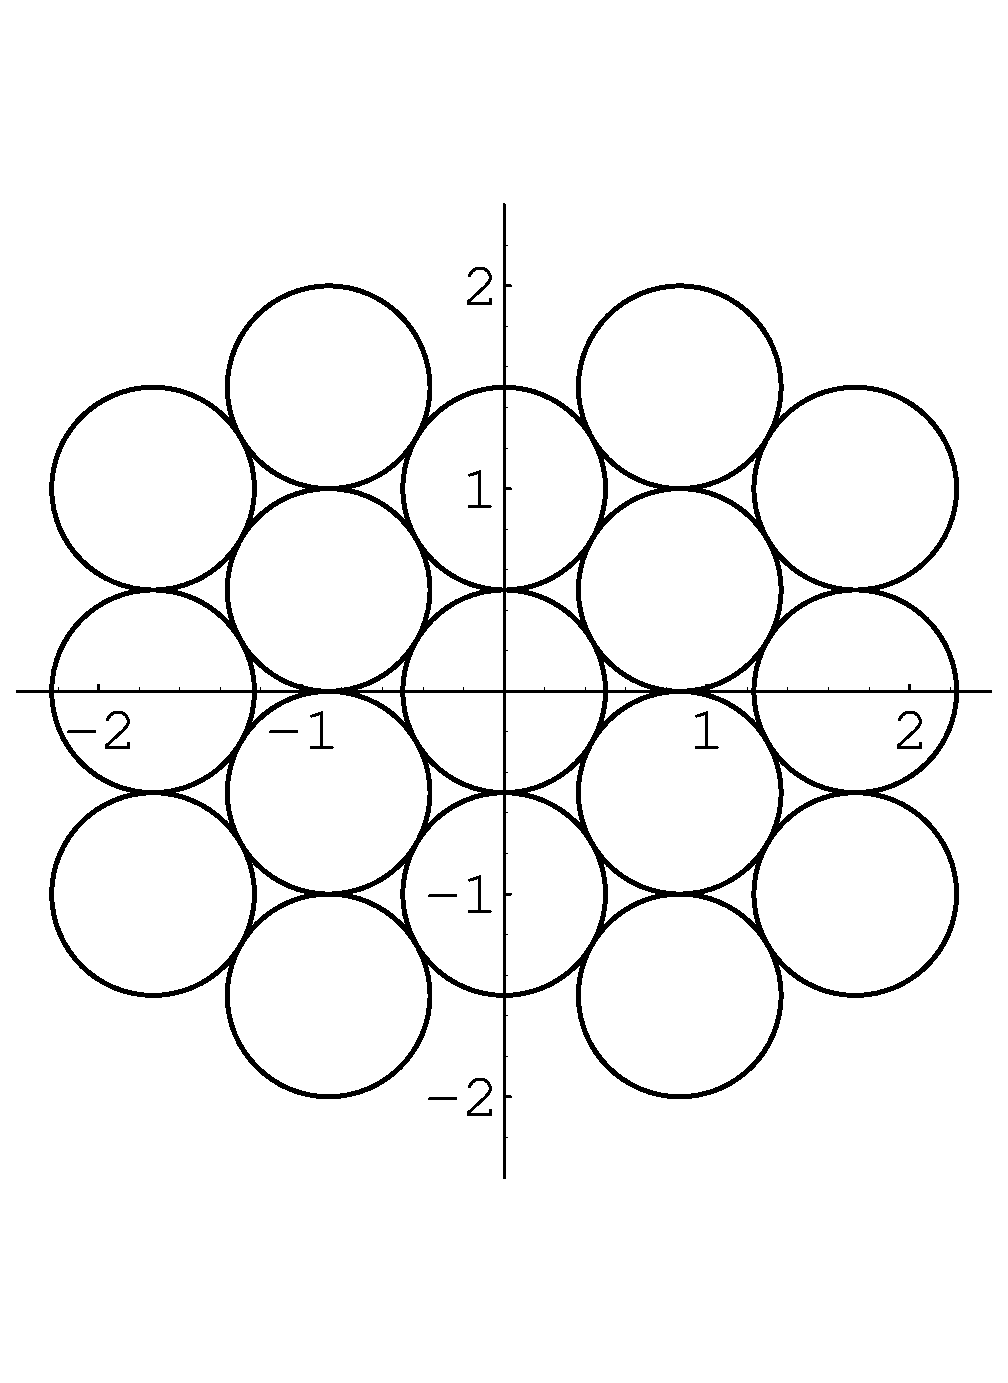
\epsfig{file=Figures/figure4.ps,height=4cm,bbllx=72pt,bblly=160pt,
bburx=540pt,bbury=630pt}
\caption{\label{f:pennies2} Staggering the pennies (or templates)
decreases the uncovered fraction of the plane to 9.3\%}
\end{center}
\end{figure}

Now suppose that we ``stagger" the pennies as shown in Figure
\ref{f:pennies2}.  In this case, the fraction of area not covered is
$\epsilon = 1 - {\pi \over 2 \sqrt{3}} =0.093\cdots$ or about 9.3\%. If
we wish to completely cover the missing bits of the plane, then we can
do so by increasing the radius of each penny by $\sqrt{5/4}$ (or,
equivalently, by moving the points at which the pennies lie closer
together by that same factor).  The resulting diagram is shown in
Figure \ref{f:pennies3}.  By increasing the number-density of pennies
on the plane by 25\% we have successfully covered up the remaining
9.3\% of the area.

\begin{figure}[h]
\begin{center}
\epsfig{file=Figures/figure5.ps,height=4cm,bbllx=72pt,bblly=160pt,
bburx=540pt,bbury=630pt}
\caption{ \label{f:pennies3} Decreasing the spacings of the pennies (or
templates) by a factor of $(5/4)^{1/2}=1.118\cdots$ then covers the
entire plane.}
\end{center}
\end{figure}

Now it is not possible to implement this algorithm exactly, because we
are not attempting to cover the entire plane, but rather only a finite
region of it.  You might think that we could just start laying down
templates in the same was as for Figure \ref{f:pennies3} and stick in a
few extra ones for any parts of the parameter space which were not
covered, but unfortunately this would then lead us to place templates
centered at points in $(\tau_0,\tau_1)$ space that do not correspond to
$\eta \le 1/4$, and for which the very meaning of a ``chirp" is
ill-defined.

The code in {\tt template\_grid()} thus uses a heuristic method to
place templates, trying whenever possible to stagger them in the same
way as Figure \ref{f:pennies3} but then shifting the center locations
when necessary to ensure that the template corresponds to physical
values of the mass parameters $m_1$ and $m_2$.  This is often referred
to as ``hexagonal packing".  In practice, to see if this placement has
been successful or not, the function {\tt plot\_template()} can be used
to visually examine the template map.

\begin{table}
\begin{tabular}[]{llllll}
Author        &   Detector             &   $f_0$/Hz     &   $\theta$/rad &   radius $ r_1$ (msec)  &   radius $r_2$ (msec)\\
\hline
Sathyaprakash &  Caltech 40m  (Nov 94) &   140          &   0.307        &    8.0                 &     0.6             \\
Owen          & Initial LIGO           &   200          &   0.5066       &    2.109               &     0.162            \\
Owen          & Advanced LIGO          &   70           &   0.4524       &    3.970               &     0.352                        
\end{tabular}
\caption{\label{t:ellipse} Orientation and dimensions of 0.97 ambiguity
templates.}
\end{table}
Table~\ref{t:ellipse} gives information about the appropriate template
sizes, spacings and orientations as found in the recent literature,
and using the {\tt match\_fit} example program.
The angle $\theta$ is the angle to the axis of the ellipse whose radius is
$r_1$, measured counterclockwise from the $\tau_0$ axis.  The
other radius (semi-axis) of the ellipse has length $r_2$.
Equation (3.16-18) of reference
\cite{Owen} do not appear to agree with Table~\ref{t:ellipse}, but that
is because the $r_i = dx_i$ of \cite{Owen} are defined by $(dx_i)_{\rm Owen}
= dl_i/\sqrt{E_i}$.  The $dl_i$ are the edge lengths of a hypercube
in dimension $N$, chosen so that if templates are centered on its
vertices, then the templates touch in the center of the cube, so that
$(dx_i)_{\rm Owen} = dl_i/\sqrt{E_i}$.  In our $N=2$ dimensional case,
this gives $r_i = dx_i=(dx_i)_{\rm Owen}/\sqrt{2}$.  Note also that in this
table, Owen and Sathyaprakash use different definitions of $f_0$,
so that their results may not be directly compared.  In Owen's case,
$f_0$ refers to the frequency of maximum sensitivity of the detector,
whereas in Sathyaprakash's case it refers to the frequency at which the
chirp first enters the bandpass of the detector.  In the case of the
November 1994 data set, we quote two different sizes an orientations
for the ellipses, depending upon the choice of $f_0$.
\begin{description}
\item{Author:}
Bruce Allen, ballen@dirac.phys.uwm.edu
\item{Comments:}
This routine evolved from {\tt grid4.f}, which was written by Sathyaprakash.
The method used to stagger templates is heuristic, and could perhaps
be improved. Very small regions of the parameter space along the equal-mass
line ($\eta=1/4$) may not be covered by any templates.
\end{description}
\clearpage

\subsection{Function: {\tt plot\_template()}}
\setcounter{equation}0
{\tt void plot\_template(char *filename, struct Scope Grid, int npages, int number)}\\
This function generates a PostScript (tm) file that draws a set of templates
on top of the region of parameter space which they cover.

The arguments are:
\begin{description}
\item{\tt filename}: Input.  Pointer to a character string.  This is used as
  the name of the output file, into which postscript output is
  written.  We suggest that you use ``{\tt .ps}" as the final three
  characters of the filename.  These files
  are best viewed using GhostView.
\item{\tt Grid}:  Input.  The mass range specified by {\tt Grid} is used to
  draw an outline of the region in $(\tau_0,\tau_1)$ parameter space
  covered by the mass range, and an ellipse for each template included
  in {\tt Grid} is then drawn on top of this outline.
\item{\tt npages}: Input.  If there are more than a few templates (and
  there can be thousands, or more) it is impossible to view this
  graphical output unless it is spread across many pages.  {\tt npages}
  specifies the number of pages to spread the output across.  We suggest at
  least one page per hundred templates.
\item{\tt number}: Input.  Each template specified in {\tt Grid} is
  numbered by the field {\tt Grid.n\_tmplt}.  If {\tt number} is set to
  1, then when each ellipse is drawn in parameter space, the number of
  the template is placed inside the ellipse so that the particular
  template associated with each ellipse may be easily identified.  If
  {\tt number} is set to 0, then the templates are not identified in
  this way; each template is simply drawn as an empty ellipse.
\end{description}
\begin{figure}[h]
\begin{center}
\epsfig{file=Figures/figure6.ps,height=8cm,bbllx=72pt,bblly=72pt,
bburx=576pt,bbury=612pt}
\caption{ \label{f:plotexample} Part of some sample output from {\tt plot\_template()}. }
\end{center}
\end{figure}
Note that the output postscript file is designed to be edited if needed
to enable clear viewing of details.  Each file is broken into pages.
At the beginning of each page are commands that set the magnification
scale of each page, and determine if the page will be clipped at the
boundaries of the paper or not.  You can edit these lines in the
postscript file to enable you to ``zoom in" on part of the parameter
space, if desired.  By turning off the clipping, you can easily move
off the boundaries of a given page, if desired.  Some sample output
from {\tt plot\_template()} is shown in Figure \ref{f:plotexample}.
(In fact, this is part of the output file produced by the example
program, showing a small number of the total of 1001 templates
required).
\begin{description}
\item{Author:}
Bruce Allen, ballen@dirac.phys.uwm.edu
\item{Comments:}
Another option should be added, to print out at the center of each
template, the mass parameters $m_1$ and $m_2$ associated with the
template.
\end{description}
\clearpage

\subsection{Example: {\tt template} program}
\setcounter{equation}0
This example lays down an optimal grid of templates covering parameter
space.  It also outputs a postscript file (best viewed with GhostView)
which shows the elliptical region of parameter space covered by each
template.
\lgrindfile{Includes/template.tex}
Part of a typical picture contained in the output file {\tt
temp\_list.ps} is shown in Figure \ref{f:plotexample} (though for
different parameters than those shown above).
\clearpage

\subsection{Example: {\tt multifilter} program}
\setcounter{equation}0
This example implements optimal filtering by a bank of properly-spaced templates.
One could do this with trivial modifications of the example {\tt optimal} program
given earlier.  Here we have shown something slightly more ambitious.  The
{\tt multifilter} program is an MPI-based parallel-processing code, designed to run
on either a network of workstations or on a dedicated parallel machine.  It is
intended to illustrate a particularly simple division of labor among
computing nodes.  Each segment of data (of length {\tt NPOINT}) is broadcast
to the next available node.  That node is responsible for filtering the data
through a bank of templates, chosen to cover the mass range from {\tt MMIN}
to {\tt MMAX}.  The output of each one of these filters is a set of 11 signals,
which measure the following quantities:
\begin{enumerate}
\item
The largest signal-to-noise ratio (SNR) at the output of the filter, for the
given segment of data,
\item
The distance for an optimally-oriented source, in Mpc, at which the SNR
would be unity.
\item
The amplitude $\alpha$ of the zero-degree phase chirp matching the observed signal.
\item 
The amplitude $\beta$ of the ninety-degree phase chirp matching the observed signal.
\item
The offset of the best-fit chirp into the given segment of data
\item
The offset of the impulse into the given segment of data, which would
produce the observed output.
\item 
The time of that impulse, measured in seconds from the start of the
data segment,
\item
The time (in seconds, measured from the start of the data segment) at
which an inspiral, best fitting the observed filter output, would have
passed through the start frequency {\tt FLO}.
\item
The time (in seconds, measured from the start of the data segment) at
which an inspiral, best fitting the observed filter output, would have
passed through coalescence.
\item
The observed average value of the output SNR (should be approximately
unity).
\item
The probability, using the splitup technique described earlier, that the
observed filter output is consistent with a chirp plus stationary
detector noise.
\end{enumerate}

For completeness, we give this code in its entirety here.  We also show
some typical graphs produced by the MPE utility {\tt nupshot} which
illustrates the pattern of communication and computation for an
analysis run.  For these graphs, the analysis run lasted only about
four minutes, and analyzed about three minutes of IFO data.  We have
performed an identical, but longer run, which analyzed about five hours
of IFO ouput in just over three hours, running on a network of eight
SUN workstations.  The data is analyzed in 6.5 second segments, each of
which is processed through a set of 66 filter templates completely
covering the mass range from 1.2 to 1.6 solar masses.  For the run that
we have profiled here, {\tt STORE\_TEMPLATES} is set to 1.  This means
that each slave allocates memory internally for storing the
Fourier-transformed chirp signals; the slaves only compute these once.
However this does place demands on the internal storage space required
- in the run illustrated here each individual process allocated about
34 Mbytes of internal memory.  Another version of the code has also
been tested; in this version the slave nodes compute the filters and
Fourier transform them each time they are needed, for each new segment
of data.  This code has {\tt STORE\_TEMPLATES}  set to 0.  This is less
efficient computationally, but requires only a small amount of internal
storage.  For a given hardware configuration, the optimal balance
between these extremes, and between the amount of redundant
broadcasting of data, depends upon the relative costs of communication
and computation, and the amount of internal storage space available.

\begin{figure}
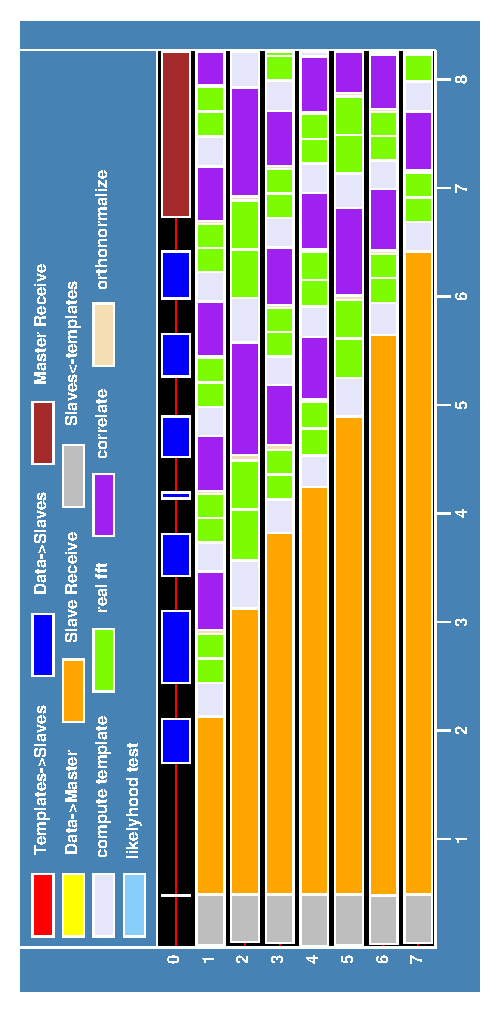
\epsfig{file=Figures/nupshot1.ps,angle=-90} 
\index{colorpage}
\caption{\label{f:nupshot1} Output of the {\tt nupshot} profiling tool,
showing the behavior of the {\tt multifilter} program running on a
workstation network of 8 machines (the fastest of these are Sparc-20
class processors).  This shows the first 8 seconds of operation (time
on the horizontal axis).  The gray segments show the slave processes
receiving the template list.  During the orange segments, the slave
processes are waiting for data; the blue segments show the master
transmitting data to each slave.  During the light gray segments, the
slaves are computing the templates, during the green segments they are
computing the FFT's of those templates, and during the purple segments
they are correlating the data against the templates.  During the brown
segment, the master is waiting to receive data back from the slaves. }
\end{figure}

\begin{figure}
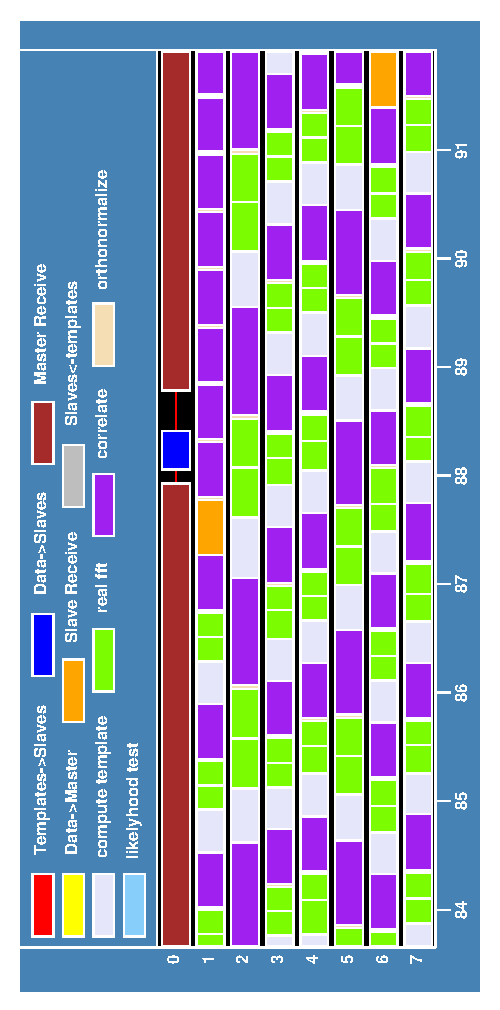
\epsfig{file=Figures/nupshot2.ps,angle=-90}
\index{colorpage}
\caption{\label{f:nupshot2} 
This is a continutation of the previous figure.  Slave number 1 has
completed its computation of the templates, and during the orange
segment, waits to make a connection with the master.  This is followed
by a (very small) yellow segment, during which the slave transmits data
back to the master, and a blue segment during which the master
transmits new data to slave number 1.  Immediately after this, slave
number 1 begins a new (purple) sequence of correlation calculations on
the newly received block of data.  Notice that because slave 1 has
already computed the templates, the light gray and green operations are
no longer needed. }
\end{figure}

\begin{figure}
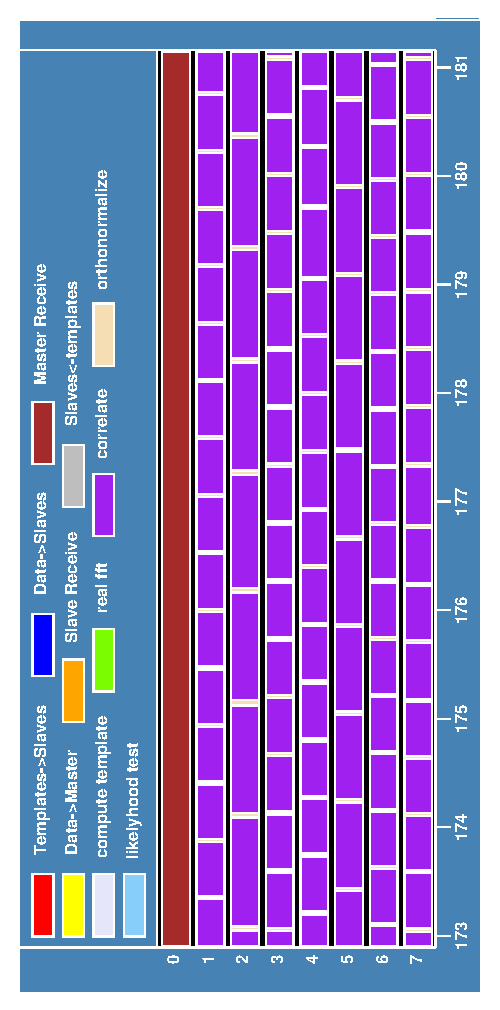
\epsfig{file=Figures/nupshot3.ps,angle=-90}
\index{colorpage}
\caption{\label{f:nupshot3} 
This is a continutation of the previous figure, and represents the
``long-term" or ``steady-state" behavior of the multiprocessing
system.  In this state, the different processors are spending all of
their time doing correlation measurements of the data, as indicated by
the purple segments, and the master is waiting for the results of the
analysis (brown segments).}
\end{figure}

\begin{figure}
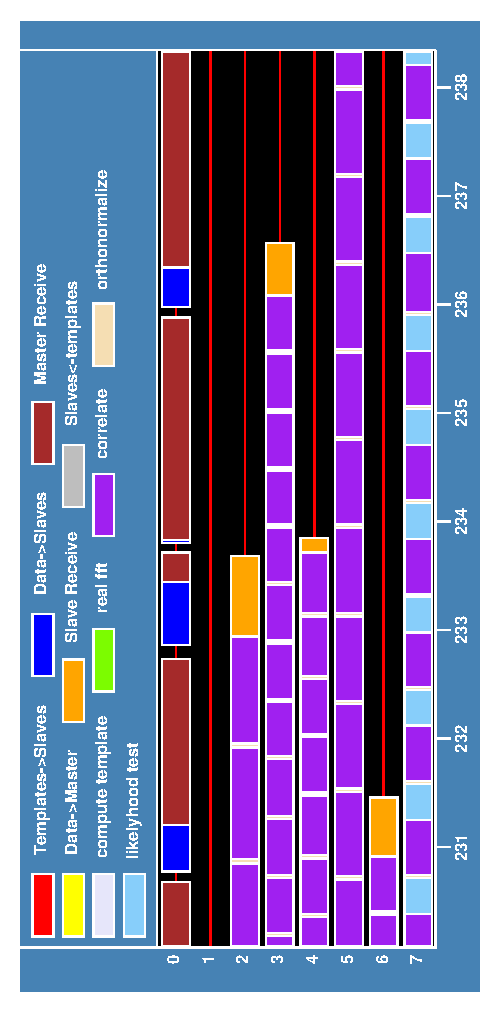
\epsfig{file=Figures/nupshot4.ps,angle=-90}
\index{colorpage}
\caption{\label{f:nupshot4} 
This is a continuation of the previous figure, and shows the
termination of some of the slave processes (all the data has been
analyzed, and there is no new data remaining).  The blue segments (data
being sent to slaves) are actually termination messages being sent to
the different processes 2,3,4 and 6.  Processes 5 and 7 are still
computing.  In the case of process 7, the data being analyzed contains
a non-stationary ``spurion" which triggered most of the filters beyond
a pre-set threshold level.  As a result, process 7 is performing some
additional computations (the split-up likelihood test, shown as light
blue segments) on the data.}
\end{figure}

Based on these figures, it is possible to provide a rough table of
computation times.  These are given in tabular form in
Table~\ref{t:compute}.

\begin{table}
\begin{tabular}[]{llll}
Task                      &   Color       &   Approximate time  & Processing done \\
\hline
data $\rightarrow$ slaves &  dark blue    &   350 msec          & transfer 384 kbytes  \\
data $\rightarrow$ master &  yellow       &   1 msec            & transfer 3 kbytes    \\
correlate                 &  purple       &   500 msec          & 2 ffts of 64k floats, and search\\
splitup (likelihood)      &  light blue   &   330 msec          & several runs through 64k floats \\
real FFT (one phase)      &  green        &   150 msec          & 1 fft of 64k floats \\
compute template          &  gray         &   350 msec          & compute 2 arrays of $\approx$ 18k floats \\
orthonormalize templates  &  wheat        &   25 msec           & several runs through 64k floats
\end{tabular}
\caption{\label{t:compute} Approximate computation times for different
elements of the optimal-filtering process.}
\end{table}

\begin{description}
\item{Author:}
Bruce Allen, ballen@dirac.phys.uwm.edu
\item{Comments:}
There are many other ways in which this optimal filtering code could be
parallelized.  This program illustrates one of the possibilities.
Other possibilities include: maintaining different templates on
different processes, and broadcasting identical IFO data to these
different processes, or parallelizing across both data and templates.
\end{description}

\clearpage
\lgrindfile{Includes/multifilter.tex}
\clearpage

\subsection{Optimization and computation-speed considerations}
\setcounter{equation}0
The previous subsection describes the {\tt multifilter} program, which
filters data through a bank of templates.  We have experimented with the
optimization of this code on several platforms, and here recount some
of that experience.

The first comment is that the {\it Numerical Recipes} routine {\tt
realft()} is not as efficient as possible.  In order to produce a
production version of the GRASP code, we suggest replacing this function
with a more-optimal version.  For example, on the Intel Paragon, the
CLASSPACK library provides optimized real-FFT functions.  To replace
the {\tt realft()} routine, we provide a replacement routine by the
same name, which calls the CLASSPACK library.  This routine may be
found in the {\tt src/optimization/paragon} directory of GRASP.  By including
the object file for this routine in the linking path, before the {\it Numerical
Recipes} library, it replaces the {\tt realft()} routine.
(Note: GRASP currently contains optimized replacement routines for
the FFT on SGI/Cray, Sun, Paragon, DEC and Intel Linux machines; see the
{\tt src/optimization/*} directories of GRASP,described in
Section \ref{ss:buildit}).

The second comment is related to inspiral-chirp template generation. The
binary inspiral chirps may be saved in the multifilter program, but
one is then limited by the available memory space, as well as incurring
the overhead of frequent disk accesses if that memory space is swapped
onto and off the disk.  To avoid this, it is attractive to generate
templates ``on the fly", then dispose of them after each segment of
data is analyzed.  This corresponds to setting {\tt STORE\_TEMPLATES}
to 0 in {\tt multifilter}.  In this instance, the computational cost of
computing binary chirp templates may become quite high, relative to the
cost of the remaining computation (FFT's, orthogonalization, searching
for the maximum SNR).

To cite a specific example, on the Intel Paragon, we found that the
template generation was almost a factor of ten more time-consuming than
the rest of the searching procedure.  Some profiling revealed that the
two culprits were the cube-root operation and the calculations of sines
and cosines.  Because the floating point hardware on the Paragon only
does add, subtract and multiply, these operations required expensive
library calls.  In both cases, a small amount of work serves to eliminate
most of this computation time.  In the case of the cube root function,
we have provided (through an {\tt ifdef INLINE\_CUBEROOT} in the code)
an inline computation of cuberoot in 15 FLOPS, which only uses add,
subtract and multiply.  This routine shifts $x$ into the range from
$1\rightarrow 2$, then uses a fifth-order Chebyshev approximation of
$x^{-2/3}$ then make one pass of Newton-Raphson to clean up to float
precision, and returns $x^{1/3} = x^{-2/3} x$.  In the case of the trig
functions we have provided (through an {\tt ifdef INLINE\_TRIGS} in the
code) inline routines to calculate the sine and cosine as well.After
reducing the range of the argument to $x\in [-\pi,\pi]$, these use
a 6th order Chebyshev polynomial to approximate the sine and cosine.
These techniques speed up the template generation to the point where it
is approximately as expensive as the remaining computations.  While there
is some small loss of computational accuracy, we have not found it to
be significant.  Shown in Figure~\ref{f:paragon} is a timing
diagram illustrating the relative computational costs of these operations.
\begin{figure}
\vskip -0.9in
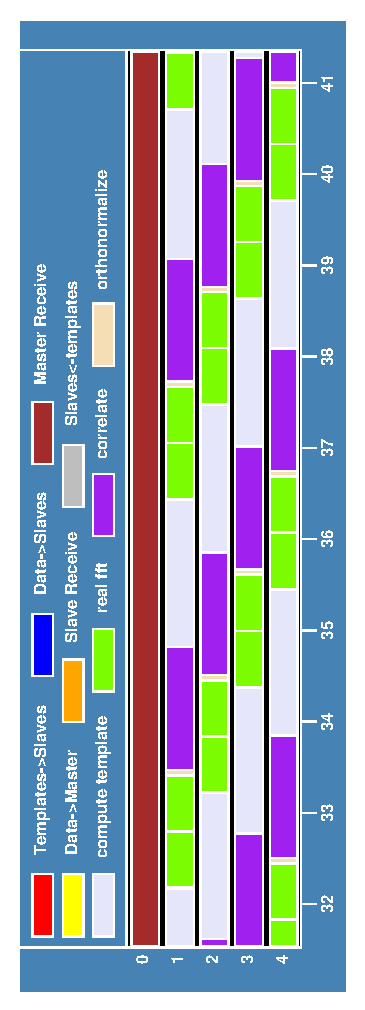
\epsfig{file=Figures/nrfft-noinline.ps,angle=-90}
\index{colorpage}
\vfill
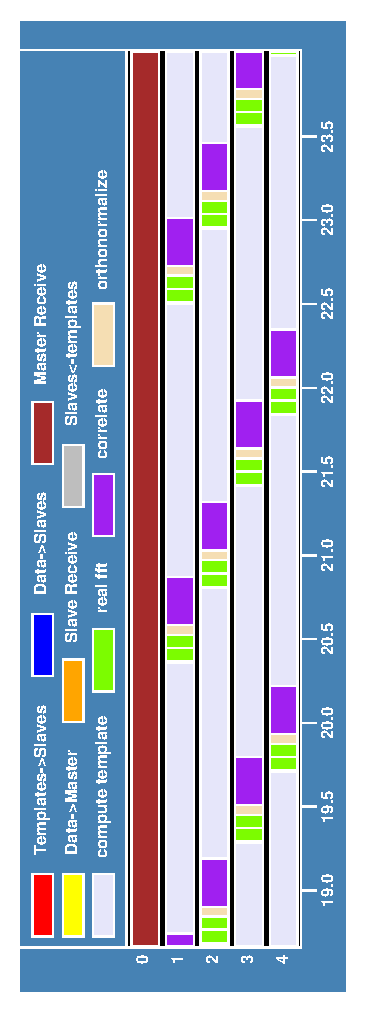
\epsfig{file=Figures/clfft-noinline.ps,angle=-90}
\index{colorpage}
\vfill
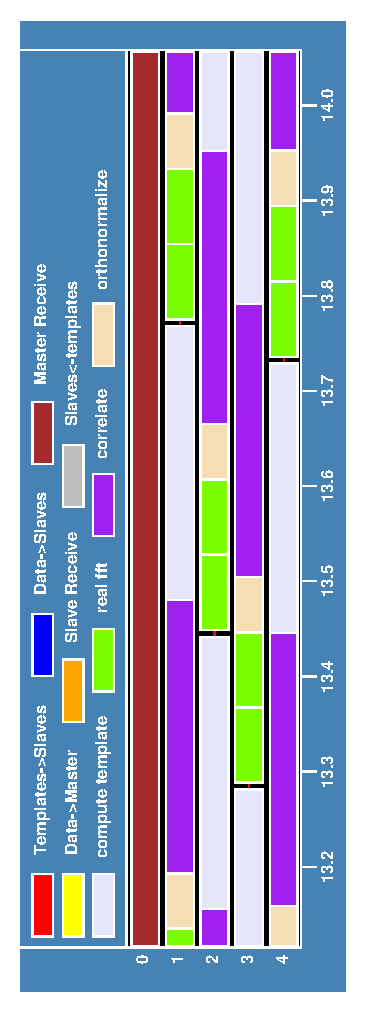
\epsfig{file=Figures/clfft-inline.ps,angle=-90}
\index{colorpage}
\vfill
\caption{\label{f:paragon} 
This shows the performance of an ``on the fly" template search on the
Intel Paragon, with different levels of optimization.  The top diagram
uses the {\it Numerical Recipes} FFT routine {\tt realft()}, and takes
about 4.2 seconds to process 6 seconds of data.  The middle diagram
shows identical code using the {\it CLASSPACK} optimized FFT routine,
and takes about 2.1 seconds.  Note that the template generation process
is now becoming expensive.  The bottom diagram shows identical code which
includes inline functions for cube-root and sine/cosine functions to speed
up the template generation process. The template generation takes about
325 msec, and the entire search procedure (including template generation)
takes 780 msec per template per processor per 6-second stretch of data.
Relative to the top diagram, this represents a speed-up factor of more
than 5.  Running on 256 nodes, it is possible to filter 5 hours of data
through 66 templates (representing the mass range from 1.2 to 1.6 solar
masses) in 5x3600x66x(0.780)/(256x6) seconds = 10.1 minutes.
}
\vskip -1.0in
\end{figure}


%%%%%%%%%%%%%%%%%%%%%%%%%%%%%%%%%%%%%%%%%%%%%%%%%%%%%%%%%%%%%%%%%%%%%%
%%%%%%%%   BEGINNING OF RESPONSIBILITY OF TEVIET CREIGHTON   %%%%%%%%%
%%%%%%%%%%%%%%%%%%%%%%%%%%%%%%%%%%%%%%%%%%%%%%%%%%%%%%%%%%%%%%%%%%%%%%

\clearpage
\subsection{Template Placement}
\label{ss:placement}

As mentioned in preceding sections, when detecting signals using a
discrete bank of templates, some loss in signal strength will always
occur due to imperfect matching of the signal with the closest
template in the bank.  The \emph{match function} $\mu$ measures this
signal loss; the \emph{mismatch} $1-\mu$ can then be thought of as a
proper distance interval on the template parameter space.  The goal of
template bank construction is to place templates with a sufficient
density in parameter space that the fractional signal loss is reduced
to less than some specified amount.  However, since each template in
the bank represents a computational investment, one would like to do
this with as few templates as possible.

Conceptually this can be thought of as a tiling problem --- one
attempts to cover the parameter space completely with ``tiles'', each
representing a template.  Each tile is small enough to fit entirely
within the equimatch contour at the specified match level, drawn about
the tile's centre.  For match levels close to 1, the match function
$\mu$ drops off quadratically with parameter offsets, and the
equimatch contours are ellipses.  However, the sizes and orientations
of these ellispes will in general vary over the parameter space, as
the behaviour of the match function changes.  This complicates the
problem significantly.  For instance, while hexagonal tiling can be
shown to be the most efficient tiling scheme when tile sizes are
constant, it is not at all clear how to implement such a scheme when
the sizes and shapes of the hexagons are allowed to vary.

For this reason, a somewhat less efficient but algorithmically simpler
tiling scheme has been adopted.  We lay out on the parameter space a
rectilinear coordinate system with some arbitrary rotation, take our
tiles to be rectangles whose sides are aligned with the coordinate
axes.  The width and height of each tile may vary so that it exactly
inscribes the equimatch ellipse, but its orientation is fixed by the
coordinate system.  As figure~\ref{f:tiling}(a) shows, aligning the
coordinate axes with the principle axes of the ellipse results in the
largest tile areas, and hence the fewest number of templates.  When
the ellipse have changing orientations, one must choose some
appropriate averaged angle for the coordinate system.  Several guesses
are often required before an optimal orientation is found.
\begin{figure}[h]
\begin{center}
\epsfig{file=Figures/fig_tiling.ps}
\caption{ \label{f:tiling}
  Some aspects of template placement using rectangular tiling: (a) By
  applying a coordinate rotation, the axes of the equimatch ellipse
  can be alligned with the axes of the rectanglular tiles, maximizing
  the tile area.  (b) Rectangular tiles can easily be stacked into
  columns, even when the match contours are varying.  (c) At the ends
  of a column, extra overlapping tiles may be required to cover the
  edges of the parameter space. }
\end{center}
\end{figure}

Once a coordinate system is chosen, the parameter space can be divided
into columns, into which the rectangular tiles are stacked.  The
height of each tile is chosen so as to stay within its equimatch
ellipse, as shown in figure~\ref{f:tiling}(b), and the column widths
may vary between columns so as to maximize the resulting tile areas.
At the boundaries of the parameter space, extra tiles may have to be
added at the corners of a column to provide complete coverage, as
shown in figure~\ref{f:tiling}(c).

The function {\tt tiling\_2d()} (section~\ref{ss:tiling_2d}) is a
generic implementation of such a rectangular tiling scheme.  It works
on nearly any parameter space on which a proper distance metric can be
defined.  The function {\tt get\_chirp\_templates()}
(section~\ref{ss:get_chirp_templates}) implements the {\tt
tiling\_2d()} algorithm for the specific case of binary inspiral
templates, using the quadratic terms of a fit to the chirp template
match function (equation~\ref{e:cubicmatch}) to define the distance
metric on the space.


\clearpage
\subsection{Structure: {\tt struct tile}}
\label{ss:tile}

For routines which lay out a mesh of tiles, a convenient data
structure for keeping track of these templates is a linked list.  Such
a structure allows new tiles to be added or inserted into the list,
without knowing in advance how many tiles are going to be generated.
The following structure stores data for a rectangular tile inscribed
within an ellipse; this is suitable for many tiling problems in which
the goal is to fill a two-dimensional space with some minimum density
of tiles.

\noindent{\tt struct tile \{}
\begin{description}
\item{\tt int flag;}
  Error codes generated while processing this tile.

\item{\tt double x;}
  The horizontal position of the patch.

\item{\tt double y;}
  The vertical position of the patch.

\item{\tt double dx;}
  The horizontal width of the patch.

\item{\tt double dy;}
  The vertical height of the patch.

\item{\tt double r1;}
  The semimajor axis of the circumscribing ellipse.

\item{\tt double r2;}
  The semiminor axis of the circumscribing ellipse.

\item{\tt double theta;}
  The angle between the x and semimajor axes.

\item{\tt struct tile *next;}
  A pointer to the next tile in the list.

\end{description}
{\tt\};}


\clearpage
\subsection{Function: {\tt tiling\_2d}}
\label{ss:tiling_2d}

\begin{verbatim}
int tiling\_2d(double *x_bound, double *y_bound, int npts,
	      int (*metric)(double , double , double *),
	      struct tile **tail, int *n_tiles);
\end{verbatim}

This is a generic routine for laying out a mesh of overlapping
rectangular tiles in a (relatively) arbitrary two-dimensional
parameter space.  The tiles are sized such that no point on the tile
is more than one unit of proper distance from its centre, where the
proper distance is computed with a metric function which can vary
arbitrarily over the parameter space.  Thus the size and shape of the
tiles can and will vary over the space.  The tiles are rectangular,
aligned with the coordinate axes, and are laid out in columns, with
extra overlapping tiles on the edges to ensure complete coverage of
the space.  The lattice of tile positions is stored as a linked list.

Note that the routine can be easily modified to lay out tiles with
non-unit proper radius.  To scale the tiles by a factor $d$, simply
multiply the metric function by a factor $d^{-2}$.

Upon successful execution, {\tt tiling\_2d()} attaches the new linked
list to {\tt (**tail).next}, updates {\tt *tail} to point to the new
tail of the list, and returns a value of 0.  It returns an error code
of 1 if it suspects that some of the columns may not be properly
filled.  It returns 2 if at any point the width of the parameter space
was more than {\tt N\_COLS} times the computed column width.  It
returns 3 if the routine terminated prematurely for any other reason
(usually because the algorithm accidentally stepped out of the
parameter space, due to imprecise interpolation of the boundary).  In
the case of error codes 2 and 3, {\tt tiling\_2d()} still attaches the
generated list onto {\tt (**tail).next} (up to the point where the
error occurred), but does not update the position of {\tt *tail}.
{\tt tiling\_2d()} will also write appropriate error messages
indicating where any errors took place, and the {\tt flag} field of
the tile on the list (at the time of the error) is set to the error
code.  A {\tt flag} value of $-1$ on any tile is a warning flag; the
tile was placed correctly, but not all of the fields were calculated.

The arguments are:

\begin{description}
\item{\tt x\_bound:}
  Input.  An array {\tt [0..npts]} storing the $x$-coordinates of {\tt
  npts} points along the boundary of the parameter space.  The array
  has length {\tt npts+1}, but the index {\tt [npts]} should refer to
  the same point as {\tt [0]}.

\item{\tt y\_bound:}
  Input.  As above, but the $y$-coordinates.

\item{\tt npts:}
  Input.  The number of points used to specify the boundary.

\item{\tt metric():}
  Input.  This function computes the three independent components of
  the distance metric matrix at a given point in parameter space.  The
  first two arguments are the $x$ and $y$ coordinates of the requested
  point, the third passes back the metric components in a
  three-element array.  The {\tt [0]}, {\tt [1]}, and {\tt [2]} metric
  components are defined in terms of the proper interval as follows:
  $$
    ds^2 = \hbox{\tt [0]}dx^2 + \hbox{\tt [1]}dxdy
         + \hbox{\tt [2]}dy^2 .
  $$
  {\tt metric()} itself should return 0, or 1 if the metric is
  undefined or not computable at the specified location.

\item{\tt tail:}
  Input/Output.  Initially points to the ``tail'' of a pre-existing
  list; the generated list is attached to {\tt (**tail).next}.  Upon
  successful completion, {\tt **tail} is updated to the new tail of
  the list.

\item{\tt n\_tiles:}
  Input/Output.  A running tally of the number of tiles in the mesh;
  it is incremented each time a tile is added (and decremented
  whenever a tile is removed).

\end{description}

The {\tt tiling\_2d()} routine makes very few assumptions about the
parameter space.  The most stringent is the assumption that the
parameter space boundary can be expressed as bivalued functions of
both $x$ and $y$; that is, both vertical and horizontal lines
intersect the boundary at no more than two points.  If a vertical line
intersects at more than two points, the routine may come to a point
where it cannot determine the location or width of a column of tiles,
and will terminate.  If a horizontal line intersects at more than two
points, the routine may not completely cover the edges of the
parameter space.  Appropriate warning or error messages are generated
in these cases.

\begin{description}
\item{Author:}
  Teviet Creighton, teviet@tapir.caltech.edu
\end{description}


\clearpage
\subsection{Function: {\tt plot\_list}}
\label{ss:plot_list}

\begin{verbatim}
int plot_list(double *x_bound, double *y_bound, int npts,
	      struct tile *head, int n_tiles, double angle,
	      double magnification, int plot_boundary,
	      int plot_tiles, int plot_ellipses, int plot_flags,
	      const char *psfile);
\end{verbatim}

This routine generates a postscript file displaying a parameter space,
the brickwork mesh of tiles covering it, and an overlapping mesh of
elliptical contours of unit proper radius, circumscribing each tile.
The function returns the number of pages of postscript output.

The arguments are:

\begin{description}
\item{\tt x\_bound:}
  Input.  The array {\tt x\_bound[0..npts]} contains the $x$
  components of a set of {\tt npts} boundary points.  Note that the
  array is of length {\tt npts+1}; the {\tt [0]} and {\tt [npts]}
  index values refer to the same point, so the array explicitly
  describes a closed boundary; however, this is irrelevant to the
  current routine.

\item{\tt y\_bound:}
  Input.  The array {\tt y\_bound[0..npts]} contains the $y$
  components of the boundary points, as above.

\item{\tt npts:}
  Input.  The number of points along the boundary.

\item{\tt head:}
  Input.  The head of the linked list of tiles to be plotted.

\item{\tt n\_tiles:}
  Input.  The number of tiles to be plotted from the list.

\item{\tt angle:}
  Input.  The angle counterclockwise from the $x$-axis of the
  parameter space to the horizontal axis of the plot.

\item{\tt magnification:}
  Input.  The scale factor of points (${}^1\!/_{72}$ of an inch) per
  unit coordinate distance in the parameter space.

\item{\tt plot\_boundary:}
  Input.  1 if boundary is to be shown, 0 otherwise.

\item{\tt plot\_tiles:}
  Input.  1 if the tile brickwork is to be shown, 0 otherwise.

\item{\tt plot\_ellipses:}
  Input.  1 if the overlapping ellipses are to be shown, 0 otherwise.

\item{\tt plot\_flags:}
  Input.  If nonzero, indicates the size of dot used to mark flagged
  tiles (in points = ${}^1\!/_{72}$ inches).  If zero, flags are
  ignored.

\item{\tt psfile:}
  Input.  The name of the postscript file created.

\end{description}

\begin{description}
\item{Author:}
  Teviet Creighton, teviet@tapir.caltech.edu
\end{description}


\clearpage
\subsection{Constants in {\tt tiling\_2d.c}}
\label{ss:tileconst}

The following constants are {\tt \#define}d in the module {\tt
tiling\_2d.c}, and are used by the routines {\tt tiling\_2d()} and
{\tt plot\_list()}.  There may be circumstances in which they might
need to be changed.

\begin{description}
\item{\tt N\_COLS} = 1\,000\,000:
  The maximum number of columns of tiles allowed in the parameter
  space.

\item{\tt N\_ROWS} = 1\,000\,000:
  The maximum number of rows of tiles allowed in any one column.

\item{\tt X\_MARGIN} = 36~points = $0.5''$:
  The horizontal separation between the left and right borders of the
  plot and the edge of the page.

\item{\tt Y\_MARGIN} = 36~points = $0.5''$:
  The vertical separation between the top and bottom borders of the
  plot and the edge of the page.

\item{\tt X\_SIZE} = 612~points = $8.5''$:
  The width of the page.

\item{\tt Y\_SIZE} = 792~points = $11''$:
  The height of the page.

\item{\tt N\_OBJ} = 797:
   The maximum number of objects which may be placed into a single
   PostScript macro.  This limitation is required in order to prevent
   errors in certain PostScript interpreters (such as Ghostscript).
   This value may be set smaller: the only effect is to generate
   additional PostScript macros containing fewer objects each.
\end{description}


\clearpage
\subsection{Structure: {\tt struct chirp\_space}}
\label{ss:chirp_space}

The following data structure, when fully assigned, contains complete
information about a region of the parameter space of chirp signals: it
describes the extent of the region, the coordinates used on it, the
behaviour of the match function over it, and the number and location
of chirp templates covering it.  It is assumed that the templates will
be placed using coordinates $x,y$ which are related to the
$\tau_0,\tau_1$ coordinates by a simple rotation; for the best
results, the $x,y$ axes should be roughly aligned with the principle
axes of the elliptical equimatch contours discussed in
section~\ref{ss:match_parab}.  The fields of this structure are:

\noindent{\tt struct chirp\_space \{}
\begin{description}
\item{\tt float m\_mn;}
  The minimum mass of a binary component in the parameter space (solar
  masses).

\item{\tt float m\_mx;}
  The maximum mass of a binary component in the parameter space (solar
  masses).

\item{\tt float ftau;}
  The reference frequency used to define the $\tau_0,\tau_1$
  coordinates.

\item{\tt float angle;}
  The angle (radians) counterclockwise from the $\tau_0$ axis to the
  $x$ coordinate axis used in placing the template patches.

\item{\tt float match;}
  The minimum match level of the covering template patches.

\item{\tt int n\_bound;}
  The number of points used to define the boundary of the region.

\item{\tt double *x\_bound;}
  An array {\tt [0..n\_bound]} containing the $x$ coordinates of the
  points defining the boundary.  The array is of length {\tt
  n\_bound+1}, but the index values {\tt [0]} and {\tt [n\_bound]}
  should refer to the same point, so as to define an explicitly closed
  polygon.

\item{\tt double *y\_bound;}
  An array {\tt [0..n\_bound]} as above, but the $y$ coordinates.

\item{\tt struct cubic\_grid grid;}
  A data structure containing coefficients of a cubic fit to the match
  function, evaluated on a grid of points in the parameter space, plus
  related information.  See the documentation for the {\tt struct
  cubic\_grid} data structure in section~\ref{ss:cubic_grid}.

\item{\tt int n\_templates;}
  The number of template patches covering the space.

\item{\tt struct chirp\_template *templates;}
  An array {\tt [0..n\_templates-1]} of data structures describing the
  positions of the covering templates.  See the next section for a
  descrition of these data structures.

\end{description}
{\tt \};}


\clearpage
\subsection{Structure: {\tt struct chirp\_template}}
\label{ss:chirp_template}

The following data structure is used to carry information about the
position of a chirp template in a variety of coordinate systems, from
the most specific computational parameters (its index in an enumerated
list) to the most general physical parameters (the masses of its
binary components).  In many cases the transformations among these
coordinates depend on additional parameters, such as the reference
frequency for the $\tau_0,\tau_1$ coordinates, or the angle between
the $\tau_0$ and $x$ axes; this global information is typically stored
in a data structure of type {\tt struct chirp\_space}
(section~\ref{ss:chirp_space}).  In addition, the following structure
contains some information about the size of the coordinate patch
covered by the template.  The fields are:

\noindent{\tt struct chirp\_template \{}
\begin{description}
\item{\tt int flag;}
  An indicator of any errors which occured while generating or placing
  this template.  At present, the following codes are recognized:
  \begin{description}
  \item{$-$1:}
    Template is incomplete; some fields could not be filled.
  \item{0:}
    No errors occured.
  \item{1:}
    Possible uncovered region of parameter space near the corners of
    this template.
  \item{2:}
    Template placement terminated prematurely at this template, due to
    a metric singularity.
  \item{3:}
    Template placement terminated prematurely at this template, for
    some other reason.
  \end{description}

\item{\tt int num;}
  The index of the template in an enumerated list, normally ranging
  from 0 to the number of templates $-1$.

\item{\tt double x;}
  The $x$ coordinate of the template in a computational Cartesian
  coordinate system.  Normally this system is related to the
  $\tau_0,\tau_1$ coordinate system by a simple rotation, so it has
  units of seconds.

\item{\tt double y;}
  As above, but the $y$ coordinate.

\item{\tt double dx;}
  The width in the $x$ direction of a rectangular patch about the
  template, which is inscribed within an equimatch ellipse.

\item{\tt double dy;}
  The height in the $y$ direction of the rectangular patch.

\item{\tt double semimajor;}
  The length of the semimajor axis of the equimatch ellipse
  circumscribing the template patch.

\item{\tt double semiminor;}
  The length of the semiminor axis of the equimatch ellipse
  circumscribing the template patch.

\item{\tt double theta;}
  The angle counterclockwise from the $x$ axis to the semimajor axis
  (radians).

\item{\tt double tau0;}
  The 0th order post-Newtonian time to coalescence (seconds).

\item{\tt double tau1;}
  The 1st order post-Newtonian correction to the time to coalescence
  (seconds).

\item{\tt double mtotal;}
  The total mass of the binary system (solar masses).

\item{\tt double mchirp;}
  The chirp mass of the system (solar masses).

\item{\tt double mred;}
  The reduced mass of the system (solar masses).

\item{\tt double eta;}
  The ratio of the reduced mass to the total mass.

\item{\tt double m1;}
  The mass of one of the binary components (by convention, the
  larger), in solar masses.

\item{\tt double m2;}
  The mass of the other binary component (by convention, the smaller),
  in solar masses.

\end{description}
{\tt \};}


\clearpage
\subsection{Function: {\tt set\_chirp\_space}}
\label{ss:set_chirp_space}

\begin{verbatim}
void set_chirp_space(struct chirp_space space);
\end{verbatim}
This routine sets a global parameter {\tt global\_space} in the {\tt
chirp\_templates.c} module, which is required for the {\tt
chirp\_metric()} routine to function --- see
section~\ref{ss:chirp_metric}.  This data must be passed to {\tt
chirp\_metric()} as a global parameter, rather than an argument, in
order for {\tt chirp\_metric()} to have a ``generic'' argument list as
required by the routine {\tt tiling\_2d()}
(section~\ref{ss:tiling_2d}).

The argument is:

\begin{description}
\item{\tt space:}
  Input.  The structure that {\tt global\_space} is set to equal.
\end{description}


\clearpage
\subsection{Function: {\tt chirp\_metric}}
\label{ss:chirp_metric}

\begin{verbatim}
int chirp_metric(double x, double y, double *m);
\end{verbatim}
This routine computes the coefficients of a local distance metric on
the space of chirp templates, at a specified location in that space.
It returns 0 upon successful completion, or 1 if the metric could not
be computed at that point.

The arguments are:

\begin{description}
\item{\tt x:}
  Input.  The $x$ coordinate of the specified point.

\item{\tt y:}
  Input.  The $y$ coordinate of the specified point.

\item{\tt m:}
  Output.  The array {\tt m[0..2]} contains the three independent
  components of the local distance metric; see below.

\end{description}

Note that this routine uses the global parameter {\tt global\_space},
defined at the top of the\\
{\tt chirp\_templates.c} module.  This
parameter must be set by the routines {\tt set\_chirp\_space()} or
{\tt get\_chirp\_templates()} before {\tt chirp\_metric()} can be
called.  The $x,y$ coordinate system used is the one defined in the
{\tt global\_space} structure: it is to a (counterclockwise) rotation
of the $\tau_0,\tau_1$ coordinate system by an angle of {\tt
global\_space.angle}.  The metric is computed by interpolating the
grid of precomputed quadratic coefficients of the match function,
stored in {\tt global\_space.grid}.

The local distance function is defined so that the match decreases to
the value {\tt global\_space.match} at a proper distance of 1.  That
is, the unit of proper distance is defined to be the maximum template
patch radius.  The metric coefficients {\tt m[0..2]} are related to
the proper interval $ds^2$ by:
\begin{equation}
  ds^2 = \hbox{\tt m[0]}dx^2 + \hbox{\tt m[1]}dxdy +
         \hbox{\tt m[2]}dy^2 \; .
\end{equation}
Note that $ds^2=1$ corresponds to the match being equal to $\mu$={\tt
global\_space.match} in equation~\ref{e:cubicmatch}.  We ignore the
cubic components of the match function when dealing with the local
distance metric.  So we have:
\begin{equation}
  \hbox{\tt global\_space.match} = 1 + \hbox{\tt coef[0]}dx^2
                                    + \hbox{\tt coef[1]}dxdy
                                    + \hbox{\tt coef[2]}dy^2
\end{equation}
when $ds^2=1$.  So the metric components {\tt m[]} are related to the match
function coefficients {\tt coef[]} via:
\begin{equation}
  \hbox{\tt m[i]} = \frac{\hbox{\tt coef[i]}}
    {\hbox{\tt global\_space.match}}\;,  \hbox{\tt i}=0 \ldots 2 \;.
\end{equation}

This routine also checks to make sure that the resulting metric is
positive definite, which should always be the case if the match
function is locally paraboloidal (rather than a saddle).

\begin{description}
\item{Author:}
  Teviet Creighton, teviet@tapir.caltech.edu
\end{description}


\clearpage
\subsection{Function: {\tt get\_chirp\_boundary}}
\label{ss:get_chirp_boundary}

\begin{verbatim}
void get_chirp_boundary(struct chirp_space *space);
\end{verbatim}
This routine computes the boundary of the triangular parameter space
of chirp signals, setting the fields {\tt x\_bound} and {\tt y\_bound}
of {\tt *space}.  Memory for these arrays is allocated in this
routine; to free it, call {\tt free((*space).x\_bound)} and {\tt
free((*space).y\_bound)}.

The argument is:

\begin{description}
\item{\tt space:}
  Input/Output.  The data structure describing the parameter space of
  chirps.  This routine uses as input the fields {\tt m\_mn}, {\tt
  m\_mx}, {\tt ftau}, {\tt angle}, and {\tt n\_bound}, and assigns the
  fields {\tt x\_bound} and {\tt y\_bound}.

\end{description}

\begin{description}
\item{Author:}
  Teviet Creighton, teviet@tapir.caltech.edu
\item{Comments:}
  The boundary is actually made to lie just inside of the triangular
  region specified by {\tt m\_mn}$<m_2<m_1<${\tt m\_mx}.  Particular
  care is taken along the equal mass line to insure that when one
  connects the computed points, the resulting line segments lie
  entirely inside the true boundary: the points must be shifted
  inwards to account for the slight concavity along this curve.  Such
  caution is required because we must occasionally convert points back
  into mass space, and bad things happen if the points lie even
  slightly past the equal mass line.
\end{description}


\clearpage
\subsection{Function: {\tt get\_chirp\_grid}}
\label{ss:get_chirp_grid}

\begin{verbatim}
int get_chirp_grid(struct chirp_space *space, const char *gridfile);
\end{verbatim}
This routine sets the field {\tt (*space).grid}, which contains
pre-computed coefficients of the cubic fit to the match function at
various points over the parameter space.  It returns 0 if no warnings
were generated, 1 if parameters used to generate the coefficient grid
differed in some nontrivial way from those of the parameter space, or
2 if the coefficient grid could not be read in; in the latter case,
{\tt (*space).grid} is unchanged.  Otherwise, this routine will
allocate memory for the coefficient grid; to free this memory, call
{\tt free\_cubic((*space).grid)}.

The arguments are:

\begin{description}
\item{\tt space:}
  Input/Output.  The parameter space over which the coefficient grid
  is being assigned.  The fields {\tt m\_mn} and {\tt m\_mx} are used
  only to check that the grid covers the space.  The fields {\tt
  ftau}, {\tt angle}, and {\tt match} are used to check, rotate, and
  rescale the grid's coordinate system (repsectively).  The field {\tt
  grid} is the one which is set by this routine.

\item{\tt gridfile:}
  Input.  The name of a file containing the pre-computed coefficients
  of the match function; see the routine {\tt generate\_cubic()} in
  section~\ref{ss:generate_cubic}.

\end{description}

\begin{description}
\item{Author:}
  Teviet Creighton, teviet@tapir.caltech.edu
\end{description}


\clearpage
\subsection{Function: {\tt get\_chirp\_templates}}
\label{ss:get_chirp_templates}

\begin{verbatim}
int get_chirp_templates(struct chirp_space *space);
\end{verbatim}
This routine computes the positions of a mesh of chirp templates on a
parameter space, using the generic tiling routine {\tt tiling\_2d()}.
See section~\ref{ss:tiling_2d} for documentation of this routine.  The
function {\tt get\_chirp\_templates()} passes to {\tt tiling\_2d()}
the boundary polygon defined by {\tt (*space).x\_bound}, {\tt
(*space).y\_bound}, and {\tt (*space).n\_bound}, as well as the
template space metric function {\tt chirp\_metric()}, then converts
the returned list of templates into the array {\tt
(*space).templates}.  The {\tt chirp\_metric()} routine requires the
parameter space to be passed to it as a global static variable named
{\tt global\_space}; this variable is set equal to {\tt *space}.  The
routine {\tt get\_chirp\_templates()} itself returns the error code
generated by the call to {\tt tiling\_2d()}; see the documentation of
that routine.  If a fatal error occurs before {\tt tiling\_2d()} is
even called, {\tt get\_chirp\_templates()} returns an error code of 3,
{\tt (*space).n\_templates} is set to 0 and {\tt (*space).templates}
to {\tt NULL}.  Otherwise, memory for the template array will be
allocated; to free this memory, call {\tt free((*space).templates)}.

The argument is:

\begin{description}
\item{\tt space:}
  Input/Output.  The data structure of the parameter space being
  filled with templates.  This routine uses as input the fields {\tt
  n\_bound}, {\tt x\_bound}, {\tt y\_bound}, and {\tt grid}, and
  assigns the fields {\tt n\_templates} and {\tt templates}.

\end{description}

\begin{description}
\item{Author:}
  Teviet Creighton, teviet@tapir.caltech.edu
\end{description}


\clearpage
\subsection{Function: {\tt plot\_chirp\_templates}}
\label{ss:plot_chirp_templates}

\begin{verbatim}
int plot_chirp_templates(struct chirp_space space,
                         double magnification, int plot_boundary,
                         int plot_patches, int plot_ellipses,
                         int plot_flags, const char *psfile);
\end{verbatim}

This routine plots a postscript file of a chirp parameter space and
the templates covering it, using the generic template-plotting routine
{\tt plot\_list()}.  See section~\ref{ss:plot_list} for documentation
on this routine.  The input parameters for {\tt plot\_list()} are
passed directly from the parameters for {\tt
plot\_chirp\_templates()}, except as follows: the boundary is taken
from {\tt space.x\_bound}, {\tt space.y\_bound}, and {\tt
space.n\_bound}, the linked list of templates is generated from {\tt
space.templates} and {\tt space.n\_templates}, and the rotation angle
of the plot is such that $\tau_0$ runs down the length of the page.
The routine {\tt plot\_chirp\_templates()} itself returns the number
of pages of postscript output.

The arguments are:

\begin{description}
\item{\tt space:}
  Input.  The data structure of the parameter space and its templates.
  This routine makes use of the fields {\tt n\_bound}, {\tt x\_bound},
  {\tt y\_bound}, and {\tt angle}; if template patches or flags are to
  be plotted, the fields {\tt n\_templates} and {\tt templates} are
  also used.

\item{\tt magnification:}
  Input.  The scale factor of points (${}^1\!/_{72}$ of an inch) per
  unit coordinate distance in the parameter space.

\item{\tt plot\_boundary:}
  Input.  1 if boundary is to be shown, 0 otherwise.

\item{\tt plot\_patches:}
  Input.  1 if rectangular brickwork of patches is to be shown, 0
  otherwise.

\item{\tt plot\_ellipses:}
  Input.  1 if the overlapping match contours are to be shown, 0
  otherwise.

\item{\tt plot\_flags:}
  Input.  If nonzero, indicates the size of dot used to mark flagged
  templates (in points = ${}^1\!/_{72}$ inches).  If zero, flags are
  ignored.

\item{\tt psfile:}
  Input.  The name of the postscript file created.

\end{description}

\begin{description}
\item{Author:}
  Teviet Creighton, teviet@tapir.caltech.edu
\end{description}


\clearpage
\subsection{Example: {\tt make\_mesh} program}
\label{ss:make_mesh}

This example program generates a template space and template bank for
a binary inspiral search.  It uses the functions {\tt
get\_chirp\_boundary()} to compute the perimeter of the template
space, {\tt get\_chirp\_grid()} to read in precomputed match
coefficients over that space, {\tt get\_chirp\_templates()} to place
the template bank, and {\tt plot\_chirp\_templates()} to plot a
PostScript file of the template space.

Note that the {\tt get\_chirp\_grid()} function requires the existence
of a match coefficient data file named {\tt
cubic\_coef\_40meter\_m=0.8-3.2.ascii}, as generated by the example
program {\tt make\_grid} in section~\ref{ss:make_grid}.

This program prints log messages to {\tt stdout}, a list of the
perimeter points (in $x,y$ coordinates) to {\tt boundary.ascii}, a
list of the template positions (in mass coordinates) to {\tt
templates.ascii}, and the PostScript image to {\tt templates.ps}.
Here is the standard output produced by this program when everything
functions normally:

\begin{verbatim}
make_mesh: get_chirp_templates generated 687 templates and exited with code 0.
make_mesh: plot_chirp_templates generated 8 pages of postscript output.
\end{verbatim}

Here are the first few lines of the file {\tt templates.ascii}, which
lists the positions of the templates in mass space.  The numbers in
the two columns are the $m_1,m_2$ coordinates, in solar masses.

\begin{verbatim}
2.963451 2.980348
2.941810 2.960199
2.986875 2.999635
2.918038 2.932353
2.896092 2.911018
2.895651 2.999934
2.869409 2.885002
2.847899 2.862208
...
\end{verbatim}

Figure~\ref{f:template_mesh} shows a portion of the PostScript file
{\tt templates.ps} generated by {\tt plot\_chirp\_templates()}.  The
figure is magnified by an extra factor of 2 for clearer display.

\begin{figure}[h]
\begin{center}
\epsfig{file=Figures/fig_template_mesh.ps}
\caption{ \label{f:template_mesh}
  A portion of the chirp template parameter space generated by the
  program {\tt make\_mesh}, showing the template patches which cover
  the space to a match level of 0.98.  This figure illustrates how the
  templates are stacked in columns, with additional overlapping
  patches along the boundary.  Less obvious is the fact that the
  rectangles are not of uniform size, reflecting the changing
  behaviour of the match function over the space. }
\end{center}
\end{figure}

\lgrindfile{Includes/make_mesh.tex}

\begin{description}
\item{Author:}
  Teviet Creighton, teviet@tapir.caltech.edu
\end{description}

%%%%%%%%%%%%%%%%%%%%%%%%%%%%%%%%%%%%%%%%%%%%%%%%%%%%%%%%%%%%%%%%%%%%%%
%%%%%%%%      END OF RESPONSIBILITY OF TEVIET CREIGHTON      %%%%%%%%%
%%%%%%%%%%%%%%%%%%%%%%%%%%%%%%%%%%%%%%%%%%%%%%%%%%%%%%%%%%%%%%%%%%%%%%


\newlength{\deglen}
\newlength{\seclen}
\newlength{\arcseclen}
\settowidth{\deglen}{$^\circ$}
\settowidth{\seclen}{$\mathrm{\scriptstyle s}$}
\settowidth{\arcseclen}{$''$}
\newcommand{\degdot}{%
  \makebox[\deglen]{\makebox[0pt]{$^\circ$}\makebox[0pt]{.}}}
\newcommand{\secdot}{%
  \makebox[\seclen]{\makebox[0pt]{$^{\mathrm{\scriptstyle s}}$}%
  \makebox[0pt]{.}}}
\newcommand{\arcsecdot}{%
  \makebox[\arcseclen]{\makebox[0pt]{$''$}\makebox[0pt]{.}}}

\clearpage
